\documentclass[10pt,twoside]{article}
%\usepackage[latin1]{inputenc} % para caracteres especiais como acentos
\usepackage[utf8]{inputenc}	
\usepackage{amsmath}
\usepackage{amsfonts}
\usepackage{amssymb}
\usepackage[brazilian]{RBB}
%\usepackage[brazilian]{babel}
%\usepackage{amsthm,amsopn,amsxtra,latexsym,dsfont} % tipos de fonte forma matematica
%\usepackage{graphicx}%\usepackage{multirow}
%\usepackage[brazil]{babel}
%\usepackage[ansinew]{inputenc}
%\usepackage{url}
\usepackage{bm}  % colocar em negrito nas fórmulas
\usepackage{longtable} % Tabelas Longas com Quebra de Página
\usepackage{subfigure} % inserir imagem um do lado da outra

\usepackage{setspace}  % trocar espaçamentos do documento
\singlespace           %\singlespace and \doublespace Observações para espaçamentos específicos no texto devemos

\usepackage{tabularx}
\usepackage{placeins}

\usepackage{ragged2e}

 \unespjournalvolume{xx}
 \unespjournalnumber{x}
 \unespjournalyear{20xx}
 \unespjournalpages{1-10}

\setcounter{page}{1}

%%%%%%%%%%% Comandos criados
\newtheorem{teo}{Teorema}%[chapter] %Gera o espaço para o teorema%
\newtheorem{defi}{Definição}%[Chapter]
\newtheorem{cor}{Corolário}%[chapter]
\newcommand{\R}{\mathds{R}}

\begin{document}
	
	\title{O ENVELHECIMENTO POPULACIONAL NOS MUNICÍPIOS DO SUL/SUDOESTE DE MINAS GERAIS: ANÁLISE DE AGRUPAMENTO}
	\author{Larissa Gonçalves SOUZA\thanks{%
			Universidade Federal de Alfenas, Instituto de Ciências Exatas, Departamento, Caixa Postal, CEP: 37130-000, Alfenas, Minas Gerais, Brasil. E-mail: {\it larissa.unifal@gmail.com}} \and
		Patrícia de Siqueira RAMOS\thanks{%
			Universidade Federal de Alfenas, Instituto de Ciências Sociais Aplicadas, Departamento, Caixa Postal, CEP: 37048-395, Varginha, Minas Gerais, Brasil. E-mail: {\it siqueirapaty@gmail.com}}
		\and Lincoln Thadeu Gouvêa de FRIAS\thanks{Universidade Federal de Alfenas - Unifal/MG, Instituto de Ciências Sociais Aplicadas, Departamento, Caixa Postal, CEP: 37048-395, Varginha, Minas Gerais, Brasil. E-mail: {\it lincolnfrias@gmail.com}} }
	\maketitle
	
	\begin{resumo}
	O objetivo desse trabalho foi classificar os municípios da mesorregião Sul/Sudoeste de Minas Gerais em relação ao processo de envelhecimento populacional e, especificamente, identificar os grupos de municípios mais e menos envelhecidos. As variáveis selecionadas para o estudo foram: esperança de vida ao nascer, taxa de fecundidade total, mortalidade infantil, mortalidade até 5 anos de idade, razão de dependência, probabilidade de sobrevivência até 40 anos, probabilidade de sobrevivência até 60 anos e taxa de envelhecimento. Esses dados são provenientes do Censo Demográfico de 2010 do IBGE, consultados por meio do Atlas do Desenvolvimento Humano no Brasil.
	Primeiro foi usado o método de Ward para definir o número de grupos, enquanto os centróides iniciais foram selecionados de forma aleatória. Em seguida, o método não hierárquico das $k$-médias foi aplicado para identificar os grupos de municípios com características semelhantes. Os resultados apontam para classificação dos municípios em quatro grupos, em relação ao processo de envelhecimento populacional.
	
\end{resumo}
	
	\begin{palavra:chave}
Análise de agrupamento; classificação; transição demográfica.	\end{palavra:chave}
	
	\section{Introdução}
Nas últimas décadas, o Brasil tem passado de forma gradual e progressiva a apresentar uma nova configuração de seu regime demográfico, caracterizado pelo envelhecimento populacional, que corresponde ao aumento, em termos relativos, da população idosa (CAMARANO, 2014). De forma geral, todo o país antes do início do processo de transição demográfica, possuía um perfil demográfico representado por muitas mortes e muitos nascimentos, resultando em um baixo crescimento vegetativo (diferença entre as taxas de natalidade e mortalidade) e população predominantemente jovem. Iniciada a transição demográfica, primeiro a mortalidade e, em seguida, a fecundidade declinam, acarretando um alto crescimento populacional. Posteriormente, na sua etapa final, o crescimento é lento novamente, mas agora movendo-se para um cenário de baixa fecundidade, aumento da longevidade e população envelhecida (LEE, 2003).

Nas próximas décadas é esperado que o envelhecimento populacional se acentue no Brasil. A velocidade com que esse fenômeno acontece nos países em desenvolvimento é considerada preocupante. Isso ocorre porque os países desenvolvidos iniciaram o processo muito antes e de maneira mais lenta (LIMA-COSTA; VERAS, 2003).
Portanto, a maioria deles teve tempo pra se ajustar à nova realidade de um país de idosos. A França e a Suécia, por exemplo, levaram, respectivamente, 115 anos e 85 anos para a proporção de idosos, com 65 anos e mais de idade, aumentar de 7\% para 14\%. Nos países em desenvolvimento, por sua vez, o cenário é diferente. No Brasil, a população idosa dobrou sua proporção de 7\% para 14\% em apenas 21 anos (DOBRIANSKY; SUZMAN; HODES, 2007). Esses dados mostram que, ainda que todos os países estejam passando por profundas transformações que levam ao envelhecimento populacional, o fenômeno não ocorre de forma homogênea. O processo se inicia em momentos, magnitude e velocidade diferentes. Isso pode ser observado não só entre países distintos, mas também dentro de um mesmo país, pois o processo é desigual em relação a suas regiões, estados e municípios.  

A importância de estudar esse fenômeno por região encontra-se no fato de que, de forma geral, o envelhecimento populacional exige uma redefinição de políticas públicas direcionadas para essa nova dinâmica demográfica. O rápido crescimento de um segmento populacionaL não produtivo e o menor crescimento do segmento produtivo podem desiquilibrar a divisão de recursos na sociedade, gerando sérios problemas econômicos. A evolução do fenômeno reforça a preocupação com os desafios gerados à saúde e assistêncial social (CARVALHO; WONG, 2008).  Nesse contexto, é necessário conhecimento sobre todos os aspectos do problema de forma a caracterizar sua magnitudade e características, que apoiarão as decisões sobre a alocação de recursos nesse novo cenário demográfico.

Atualmente, há razoável disponibilidade de dados demográficos de municípios do Brasil, relacionados ao envelhecimento, principalmente através de pesquisas do Instituto Brasileiro de Geografia e Estatística (IBGE) (em especial, os Censos Demográficos e o Perfil dos Estados e dos Municípios Brasileiros). Porém, na maior parte das vezes, as variáveis disponíveis nesses bancos de dados são analisadas separadamente e uma visão geral pode ficar comprometida. Por isso, a análise multivariada é fundamental para a análise dos dados municipais, uma vez que a realidade dos municípios é multidimensional e muitas dessas variáveis estão intimamente relacionadas. 

Nesse sentido, o objetivo deste trabalho é classificar os municípios da mesorregião Sul/Sudoeste de Minas Gerais em relação ao processo de envelhecimento populacional. Especificamente, identificar os grupos de municípios mais envelhecidos e menos envelhecidos. 



\medskip
	
\section{Dados e metodologia}
\medskip

\subsection{Dados}

As bases de dados utilizadas neste trabalho são provenientes do Censo Demográfico 2010 realizado pelo IBGE, consultado a partir do Atlas do Desenvolvimento Humano no Brasil 2013 (disponível em www.atlasbrasil.org.br). Os dados estão tabulados em formato de planilhas, o que facilita seu tratamento. Para o desenvolvimento do trabalho foram escolhidas 8 variáveis demográficas, referentes aos 146 municípios da mesorregião Sul/Sudoeste de Minas Gerais (SSM). A seguir são apresentadas essas variáveis, que têm seu comportamento relacionado em alguma medida com o processo de transição demográfica, que conduz ao envelhecimento populacional.

%Essa mesorregião foi escolhida por ser onde os três \textit{campi} da Universidade Federal de Alfenas (Unifal-MG) se encontram e com base na caracterização da mesorregião, que será apresentada mais adiante. 

\begin{itemize}
    \item {Esperança de vida ao nascer (espvida): número médio de anos que um indivíduo espera viver a partir do nascimento, se permanecerem constantes ao longo da vida o nível e o padrão de mortalidade por idade prevalecentes no ano do Censo.}

    \item {Taxa de fecundidade total (tft): número médio de filhos que uma mulher deverá ter ao terminar o período reprodutivo, que compreende o grupo etário de 15 a 49 anos de idade.}

    \item {Mortalidade infantil (mort1): número de crianças que morrem antes de completar um ano de vida em cada 1000 crianças nascidas vivas.}

    \item {Mortalidade até os 5 anos de idade (mort5): probabilidade de morrer entre o nascimento e a idade exata de 5 anos, por 1000 crianças nascidas vivas.} 

    \item{Razão de dependência total (rdt): medida pela razão entre o número de pessoas com 14 anos ou menos e de 65 anos ou mais de idade (população considerada inativa) e o número de pessoas com idade de 15 a 64 anos (população potencialmente ativa) multiplicado por 100. O indicador mede, em termos relativos, a parcela da população potencialmente inativa (dependente) que deve ser sustentada pela potencialmente ativa.}

    \item {Probabilidade de sobrevivência até 40 anos (sobre40): probabilidade de uma criança recém-nascida viver até os 40 anos, se permanecerem constantes ao longo da vida o nível e o padrão de mortalidade por idade do ano do Censo.}

    \item {Probabilidade de sobrevivência até 60 anos (sobre 60): probabilidade de uma criança recém-nascida viver até os 60 anos, se permanecerem constantes ao longo da vida o nível e o padrão de mortalidade por idade do ano do Censo.}

    \item {Taxa de envelhecimento (t\_env): razão entre a população de 65 anos ou mais de idade e a população total multiplicado por 100.}

\end{itemize}

O aumento da longevidade, representado pelos ganhos no indicador esperança de vida, ocorre como consequência da redução dos níveis de mortalidade (CARVALHO; GARCIA, 2003). Portanto, é razoável dizer que quanto menor o nível de mortalidade de um município, maior será sua esperança de vida ao nascer. Além disso, esse aumento da longevidade se deve em grande parte à redução da mortalidade infantil (CAMARANO, 2014). Isso acontece porque em um primeiro momento a queda da mortalidade se concentrou nas idades mais jovens (CARVALHO; GARCIA, 2003). Portanto, à medida que se caminha no processo de transição demográfica, menores são os níveis de mortalidade infantil e de mortalidade até os 5 anos de idade. Ao mesmo tempo, a diminuição da mortalidade que de forma geral tem atingido todos os grupos etários, leva ao aumento tanto da probabilidade de sobrevivência até os 40 anos de idade, como até os 60 anos. 

Outra componente que reduz de forma sustentada no processo de transição demográfica é a fecundidade, esse comportamento conduz ao início do processo de envelhecimento populacional (CARVALHO; WONG, 2008). Portanto, quanto menor a taxa de fecundidade total, mais envelhecido se torna o município. As variáveis razão de dependência total e taxa de envelhecimento também estão associadas à fecundidade. 


Um aumento ou queda na razão de dependência total pode ser resultado tanto de uma mudança na razão de dependência dos jovens, como na razão de dependência dos idosos. Segundo Paiva e Wajnman (2005), no processo de transição demográfica é possível identificar 3 estágios diferentes relacionados ao comportamento da razão de dependência total, devido às mudanças da estrutura etária da população. Na primeira fase da transição demográfica, a queda da mortalidade infantil gera um aumento na proporção de jovens na população e, consequentemente, contribui para o aumento da razão de dependência total, via razão de dependência dos jovens. Em um segundo estágio, ocorre uma queda da razão de dependência total, impulsionada pela redução da fecundidade, que provoca a redução da proporção de jovens na população. Portanto, nesses dois primeiros momentos, as modificações na razão de dependência total são impulsionadas, em grande parte, pela razão de dependência dos jovens.

Em todo esse período, a razão de dependência de idosos é pequena e exerce pouco peso sobre a razão de dependência total. Contudo, com a contínua queda do nível de fecundidade e aumento da proporção da população em idade avançada, a razão de dependência dos idosos irá aumentar, ultrapassando a de jovens e conduzindo ao aumento da razão de dependência total. Esse terceiro estágio vai ocorrer quando a população estiver muito envelhecida. Em relação à taxa de envelhecimento, nesse contexto ela está representando a proporção da população de 65 anos ou mais na população. Ou seja, quanto maior seu valor maior a proporção de idosos naquele município.


\medskip

\subsection{METODOLOGIA}\label{ME}

Nesse trabalho foi utilizada a técnica multivariada de análise de agrupamento para identificar os grupos de municípios da mesorregião SSM com características semelhantes. As análises foram feitas usando a linguagem $R$ (R Core Team, 2016) por meio do programa \textit{RStudio} (RStudio Team, 2016). Inicialmente foi realizada uma análise exploratória dos dados que auxiliou na aplicação das técnicas de agrupamento. Primeiro foi obtido um resumo estatístico das variáveis estudadas e, em seguida, foram apresentados os municípios com os três melhores e piores desempenhos nessas variáveis. A fim de identificar os pares de variáveis mais associadas entre si, foi calculada a matriz de correlações entre as variáveis, duas a duas, dada por

\begin{equation}\label{R}
        \boldsymbol{R} =
        \left[
        \begin{array}{cccc}
        1      & r_{12} & \dots & r_{1p} \\
        r_{21} & 1      & \dots & r_{2p} \\
        \vdots & \vdots & \ddots & \vdots \\
        r_{p1} & r_{p2} & \dots & 1 \\
        \end{array}
        \right],
\end{equation}
em que $r_{ij} = \dfrac{S_{ij}}{\sqrt{S_{ii}S_{jj}}}$ (FERREIRA, 2011).

De acordo com Hair et al. (2009), existem suposições como a normalidade, linearidade e homecedasticidade que devem ser avaliadas na análise multivariada. No entanto, algumas técnicas são mais afetadas do que outras caso ocorra violação de alguma delas. No caso da análise de agrupamento, essas suposições não possuem tanta importância, pois exercem pouco peso sobre a análise. Os autores ressaltam ainda que, no uso de técnicas de agrupamento, especial atenção deve ser dada à multicolinearidade entre as variáveis estudadas. 

Após a etapa de formulação do problema, escolha das variáveis e análise exploratória dos dados, foi iniciado o processo de agrupamento. Nesse sentido, o primeiro passo consistiu em selecionar qual seria o método de agrupamento para classificar os municípios. Foi escolhido o método não hierárquico das $k$-médias que demonstra um desempenho superior aos métodos hierárquicos por ser menos afetado por \textit{outliers} e por variáveis não relevantes para o agrupamento (MOOI; SARSTEDT, 2010). Com o uso dessa técnica, cada município foi alocado no grupo cujo vetor de médias amostral (centroide) era o mais semelhante ao vetor de valores observados para o respectivo município (MINGOTI, 2005).

O procedimento de agrupamento das $k$-médias ($k$-\textit{means}) tem como principais características: aplicação do processo à matriz de dados $\boldsymbol{X}$ e número de grupos $k$ definido \textit{a priori} (FERREIRA, 2011). A técnica procura uma partição das $n$ observações em \textit{k} agrupamentos ($G_1, G_2,  \dots , G_k$), em que $G_i$ denota o conjunto de observações que está no \textit{i}-ésimo grupo e $k$ é dado por algum critério numérico de minimização. A implementação mais usada do método tenta encontrar a partição dos $n$ elementos em $k$ grupos que minimizem a soma de quadrados dentro dos grupos (SQDG) em relação a todas as variáveis. Esse critério pode ser escrito como

\begin{equation}
SQDG = \sum_{j=1}^{p}\sum_{l=1}^{k}\sum_{i \in G_l}(X_{ij} - \bar{X}_{j}^{(l)})^2,
\end{equation}
em que $\bar{X}_{j}^{(l)} = \displaystyle\frac{1}{n_i}\sum_{i \in G_l}X_{ij}$ é a média dos indivíduos no grupo $G_l$ em relação à variável $j$ (EVERITT; HOTHORN, 2011). %(EVERITT; HOTHORN, 2011, p.175).

Segundo Mingoti (2005), o processo iterativo do método pode ser descrito pelos seguintes passos: %mingoti p.192%

(1) Inicialmente são escolhidos $k$ centroides, denominados de "sementes", calculados com base no número de grupos escolhido \textit{a priori};

(2) Uma medida de distância é aplicada para comparar cada objeto a cada centroide inicial, então o objeto é unido ao grupo de menor distância;

(3) Os valores dos centroides são recalculados considerando cada grupo formado, então o passo 2 é repetido com os novos vetores de médias calculados para os novos grupos;

(4) Os passos 2 e 3 são repetidos até que não haja mais realocação dos objetos entre os grupos. 

O método das $k$-médias exige que seja definido \textit{a priori} tanto o número de grupos desejado quanto as $k$ sementes. Dentre os critérios disponíveis na literatura, encontra-se o uso de uma técnica hierárquica. Nessa abordagem primeiro uma técnica hierárquica é aplicada para identificar o número de grupos \textit{a priori} e, em seguida, são definidas as sementes iniciais e o método das k-médias é aplicado para classificar as observações. Nesse trabalho, foi escolhido o método de Ward para especificar o número de grupos pretendido. Além dele retornar melhores desempenhos que os outros métodos (EVERITT; HOTHORN, 2011), o método é considerado mais preciso e indicado dados quantitativos contínuos (BLASHFIELD, 1976). 

Diversas sugestões para a definição das sementes são apresentadas na literatura, Mingoti (2005) apresenta algumas propostas, sendo elas: aplicação de técnicas hierárquicas aglomerativas, escolha aleatória ou via observação dos valores discrepantes do conjunto de observações. Pena, Lozano e Larranaga (1999) apresentam um estudo comparativo de diferentes métodos de inicialização para as $k$-médias e a escolha aleatória aparece como um dos melhores dentre os comparados, por tornar o procedimento das $k$-médias mais efetivo e independente do agrupamento inicial. Nesse trabalho foi utilizada a função \texttt{kmeans} do \texttt{R}, sua documentação sugere a escolha aleatória das sementes iniciais e que esse número seja 25. Portanto, primeiro foi aplicado o método de Ward para definir o número de grupos e, em seguida, o método das $k$-médias para a classificação dos municípios em grupos. 

Para aplicação do método de Ward foi usada a distância de Mahalanobis, para medir o quão próximos estão dois grupos ou observações. Dessa forma, seja $\boldsymbol{S^{-1}}$ a matriz de covariâncias da matriz de dados a distância de Mahalanobis entre
dois elementos $X_{i.}$ e $X_{j.}$ é definida por:

\begin{equation}
d_{ij}= (\boldsymbol{X_{i.}} - \boldsymbol{X_{j.}})^{T} \boldsymbol{S^{-1}} (\boldsymbol{X_{i.}} - \boldsymbol{X_{j.}}).
\end{equation}

Essa medida é indicada quando as variáveis estão altamente correlacionadas, pois ela ajusta as correlações entre as variáveis e pondera igualmente cada variável do conjunto de dados original (HAIR et al., 2009). Além disso, assim como na abordagem não hierárquica, nesse caso também é necessário definir o número de grupos da partição final. Contudo, nos métodos hierárquicos aglomerativos o número é definido no final do processo de agrupamento, decidindo-se o ponto de corte do dendrograma. Diante disso, foram utilizados os critérios da maior diferença no nível de fusão e da interpretabilidade. O primeiro critério refere-se à maior altura no dendrograma, que indica que o grupo pode se tornar menos homogêneo internamente com essa união  (EVERITT et al., 2011). O segundo critério diz respeito à melhor solução cuja interpretação corresponda aos objetivos da análise.

Por fim, os grupos resultantes foram representados no mapa da mesorregião SSM com o intuito de verificar a proximidade geográfica dos municípios inseridos em cada grupo. Foram utilizados gráficos \textit{boxplots} para analisar a variabilidade dos dados estudados e comparar os grupos obtidos em relação às variáveis. O eixo horizontal do gráfico representa os grupos na ordem de 1 a 4 e o eixo vertical a variável analisada. Além disso, como suporte para avaliação dos grupos foram calculadas algumas medidas estatísticas como a mediana, o coeficiente de variação (CV), máximo e mínimo das variáveis de cada agrupamento. O CV é uma medida de dispersão relativa usada para avaliar a homogeneidade interna do agrupamento. Quanto menor seu valor, mais homogêneo é considerado o grupo em relação àquela variável. Por último, foram selecionadas as variáveis população (pop) e rendimento médio dos ocupados (renocup), com o intuito de caracterizar o comportamento dos grupos mais envelhecidos e menos envelhecidos em relação à população e renda.

\medskip


\section{\textbf{Resultados e discussão}}
	
\medskip

\subsection{Análise descritiva das variáveis}

O primeiro passo consistiu em obter um resumo estatístico das variáveis demográficas, apresentado na Tabela \ref{RE}. O resultado mostra que a menor esperança de vida ao nascer (espvida), no ano 2010, da mesorregião Sul/Sudoeste de Minas Gerais, foi 73,03 anos (Carmo da Cachoeira, Divisa Nova, São Bento Abade e São Tomé das Letras) enquanto a maior 78,15 anos (Passos). Portanto, um indivíduo nascido, em 2010, Passos, por exemplo, esperava viver em média 78,15 anos. Esses valores sinalizam um regime de baixa mortalidade e alta esperança de vida ao nascer na mesorregião estudada. 

Em relação à taxa de fecundidade total (tft), a menor registrada foi de 1,33 filhos por mulher (São Sebastião do Rio Verde e São João da Mata), ao passo que a maior foi de 2,70 filhos por mulher (São Bento Abade). Além disso, os dados mostram que pelo menos 109 dos 146 municípios estudados já experimentam taxas de fecundidade total abaixo do nível de reposição (2,1 filhos por mulher), representado pelo terceiro quartil 2,08. 

\begin{table}[!ht]
\centering
\caption{Resumo estatístico das variáveis demográficas da mesorregião Sul Sudoeste de Minas Gerais, 2010.}
\label{RE}
\[ \begin{tabular}{lrrrrrrrrr}
\hline
& espvida & tft  & mort1 & mort5 & rdt    & sobre40 & sobre60 & t\_env   \\ \hline
mínimo    & 73,03   & 1,33 & 10,35 & 12,11 & 37,68 & 92,33   & 79,54   & 5,46      \\
1 quartil & 74,44   & 1,79 & 13,40 & 15,63 & 43,26 & 93,23   & 81,67   & 8,49      \\
mediana   & 75,56   & 1,95 & 14,45 & 16,86 & 44,85 & 93,92   & 83,32   & 9,39     \\
média     & 75,46   & 1,95 & 14,69 & 17,09 & 45,24 & 93,85   & 83,15   & 9,45     \\
3 quartil & 76,28   & 2,08 & 16,18 & 18,86 & 47,27 & 94,35   & 84,36   & 10,32    \\
máximo    & 78,15   & 2,70 & 18,50 & 21,55 & 53,20 & 95,99   & 87,58   & 14,85   \\ \hline
\end{tabular} \]
\end{table}
\FloatBarrier


Uma das maneiras de medir a relação intergeracional dos municípios é por meio da razão de dependência total (rdt). Quanto maior a razão, maior o peso da população considerada inativa (0 a 14 anos e 65 anos e mais de idade) sobre a população ativa (15 a 64 anos de idade). A mediana mostra que 50\% dos valores estão abaixo de 44,85. O menor valor do indicador encontrado registrou 37,68 dependentes para cada 100 pessoas potencialmente ativas (Tocos do Moji) e o maior atinge 53,20 dependentes (São Tomás de Aquino). A razão de dependência total é formada pela soma entre a razão de dependência dos jovens e a razão de dependência dos idosos. Quando o Brasil era caracterizado por um regime de alta fecundidade e redução da mortalidade, a razão de dependência dos jovens tinha um peso muito maior que a dos idosos. Atualmente, com a queda das taxas de fecundidade e o consequente envelhecimento da população, é razoável dizer que a razão de dependência dos idosos tem sido a principal responsável pelos aumentos observados na razão de dependência total.  

Em relação ao indicador mortalidade infantil (mort1), o menor valor registrado é 12,11 (Passos) que corresponde ao número de crianças que morreram antes de completar um ano de vida em cada 1000 crianças nascidas vivas. A maior taxa de mortalidade infantil foi de 18,50 óbitos por mil nascidos vivos registrada pelos municípios de Carmo da Cachoeira, Divisa Nova, São Bento Abade e São Tomé das Letras. A mortalidade até os 5 anos de idade (mort5), por sua vez, registrou o valor de 12,11 como o mínimo e 21,55 como o máximo. Como a mortalidade infantil está contabilizada na mortalidade até os 5 anos de idade, os municípios associados aos maiores e menores valores desse indicador são os mesmos para os dois casos. Além disso, os menores níveis de mortalidade podem ser associados a maior longevidade. Os municípios de Passos e Itajubá, por exemplo, apresentam os menores níveis de mortalidade e são responsáveis pelas maiores esperanças de vida ao nascer. 

A maior probabilidade de sobrevivência até 40 anos de idade encontrada na mesorregião estudada é 0,96 (Itajubá e São Lourenço), ao passo que a menor é 0,92 (Natércia). Em relação a probabilidade de sobrevivência até 60 anos de idade, o maior valor registrado é 0,87 (Itajubá e São Lourenço) e o menor é 0,80 (Natércia). Em relação à taxa de envelhecimento, a mediana do indicador foi de 9,39\%, sendo o valor máximo 14,85\% (Córrego do Bom Jesus) e o mínimo 5,46\% (Senador Amaral). Além disso, 109 dos 146 municípios estudados experimentam taxa de envelhecimento menores que 10,32\%. A taxa de participação dos idosos (65 anos ou mais de idade) em relação a população total do município. Uma taxa elevada reflete, principalmente, a redução dos níveis de fecundidade e o aumento da esperança de vida dos idosos. De forma geral, é razoável dizer que aqueles municípios com os melhores indicadores estão em um estágio mais avançado da transição demográfica, registrando menores níveis de mortalidade e fecundidade. 

O próximo passo da análise exploratória do conjunto de dados foi a análise da correlação entre as variáveis. A Figura \ref{cor} apresenta as correlações entre cada um dos pares de variáveis demográficas selecionadas, antes e após a retirada de variáveis. Quanto maior o diâmetro do círculo, mais próximo de 1 é o valor do coeficiente de correlação e, portanto, maior o grau de associação entre as variáveis. Em relação às cores, a associação positiva é indicada pela cor azul e a negativa pela cor vermelha. 

\begin{figure}[htp!]

\center
\subfigure[ref1][Antes]{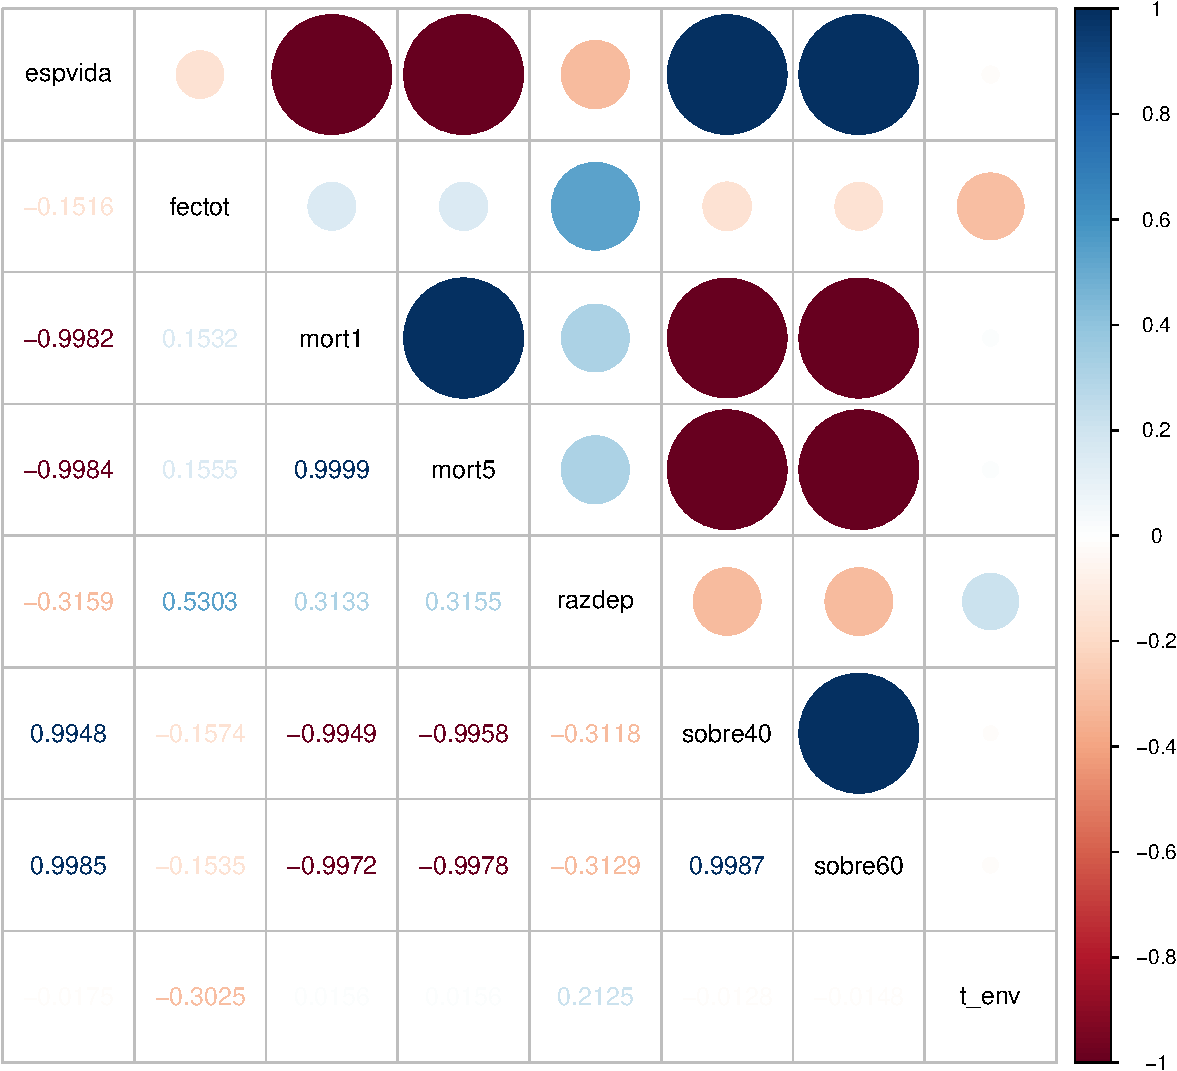
\includegraphics[width=5cm]{corrplot_todas}}
\qquad
\subfigure[ref2][Depois]{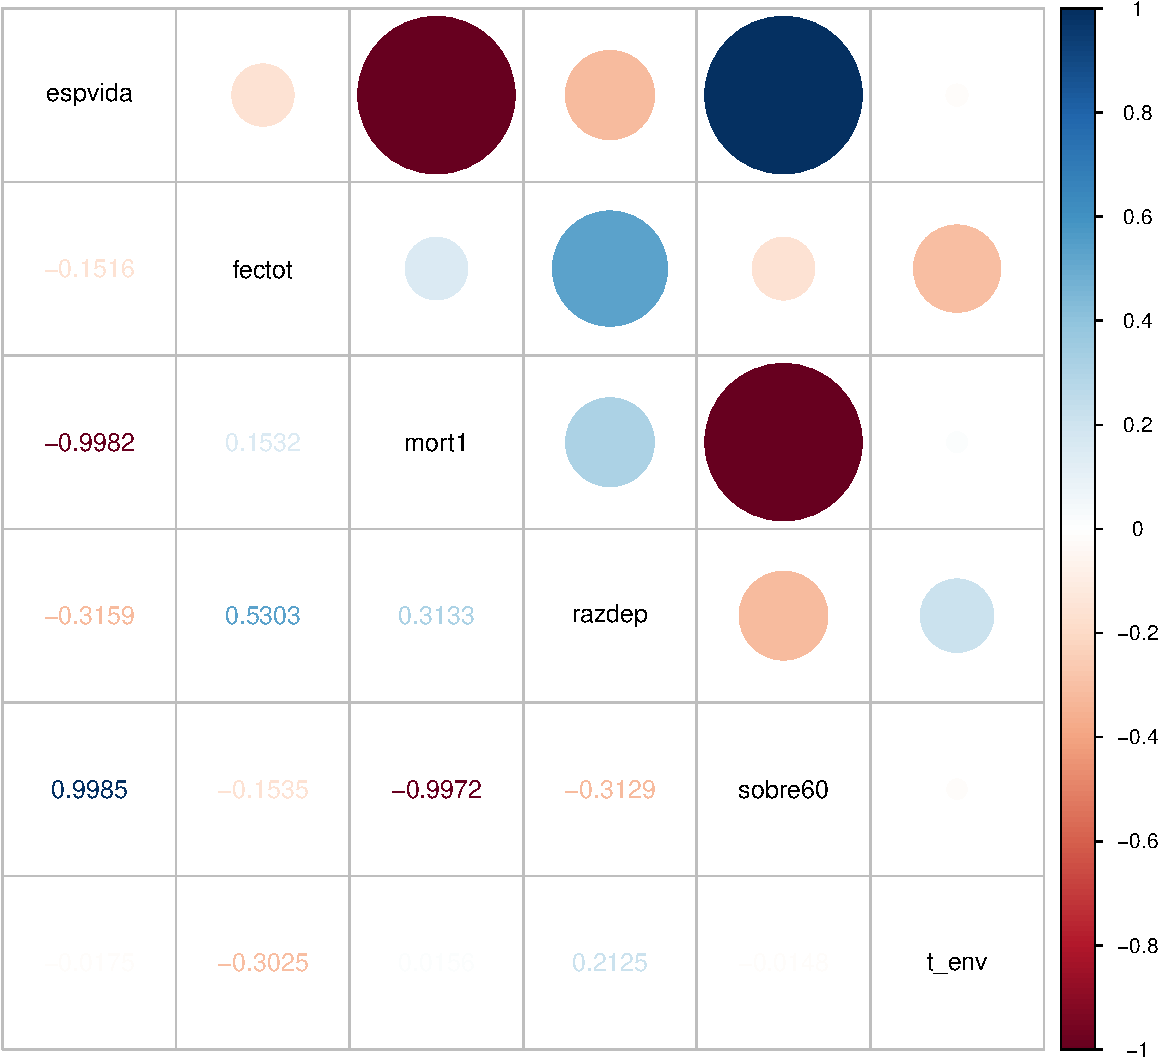
\includegraphics[width=5cm]{corrplot_utiliz}}
\caption{Correlações entre as variáveis (antes e após a retirada de variáveis).}
\label{cor}
\end{figure}
	
A variável espvida é correlacionada negativamente com as variáveis mort1 e mort5 e positivamente com as variáveis sobre40 e sobre60. Quanto menor a mortalidade, maior é a esperança de vida ao nascer e quanto maior a probabilidade de sobrevida, maior a esperança de vida ao nascer. As variáveis mort1 e mort5 apresentam correlação de 0,9999, ou seja, quanto maior a mortalidade infantil, maior será a mortalidade até os 5 anos de idades. Do mesmo modo, essas variáveis são correlacionadas negativamente com as probabilidades de sobrevida até aos 40 e 60 anos. As variáveis sobre40 e sobre60 também apresentam alta correlação (0,9987). Por fim, as variáveis tft e rd estão positivamente correlacionadas. Isso pode estar associado ao fato de que a menor tft, em um primeiro momento, reduz a razão de dependência dos jovens, o que conduz à redução da razão de dependência total. 

De forma geral, as variáveis da análise são altamente correlacionadas. As maiores correlações encontradas foram entre as variáveis sobre40 e sobre60, bem como entre mort1 e mort5. Nesse sentido, foi necessário fazer a escolha de quais variáveis permaneceriam na análise. Como mort1 e mort5 representam informações sobre nível de mortalidade, foi decidido retirar mort5 da análise porque a mortalidade infantil é considerada mais representativa nesse contexto. Do mesmo modo, sobre60 permaneceu no estudo por ser considerada mais informativa que sobre40. As demais variáveis, apesar de apresentarem altas correlações, continuaram na análise porque elas representam informações interessantes, que poderiam ser úteis para os agrupamentos.


\subsection{Agrupamentos}

Inicialmente, com o intuito de visualizar a existência de possíveis agrupamentos nos dados, foram ilustrados os dois primeiros componentes principais nos eixos horizontal e vertical da Figura \ref{cps1}. Dessa forma, cada município foi representado pelo seu valor numérico dos componentes, os chamados escores. Os dois primeiros componentes principais explicaram 76\% da variância total. Além disso, é possível observar que muitas observações (municípios) ficaram posicionadas muito próximas e outras mais distantes entre si. No entanto, a disposição dos municípios no gráfico não deixa claro a divisão das observações entre grupos. 


\begin{figure}[htp!]
\begin{center} 
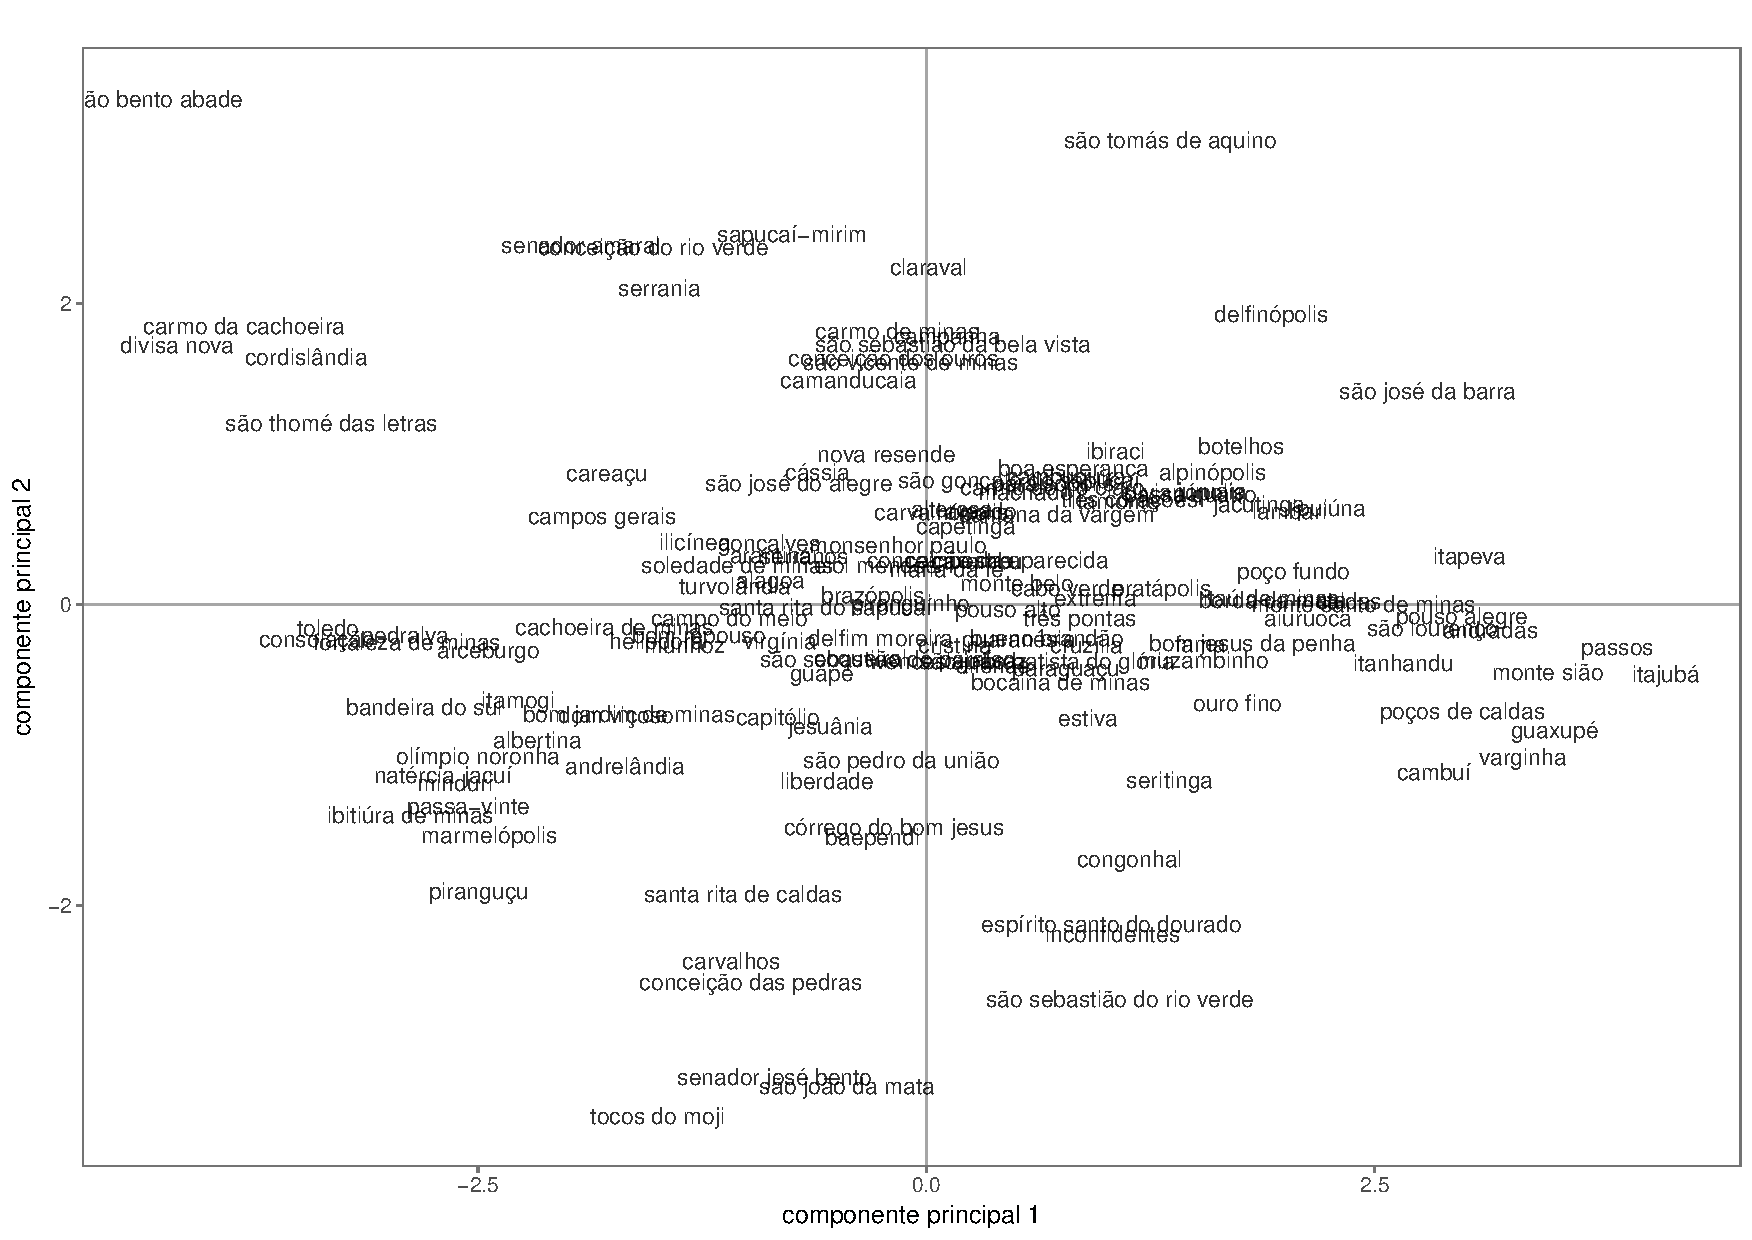
\includegraphics[scale=0.24]{dispersao_CPs}
\end{center}
\caption{Dispersão dos municípios em função dos escores dos componentes principais.} \label{cps1}
\end{figure}
\FloatBarrier

Em seguida, foi obtido o dendrograma da análise de agrupamento pelo método de Ward e distância de Mahalanobis, apresentado na Figura \ref{wr_maha}. O corte foi realizado na altura que classifica as observações em quatro agrupamentos. Também foram examinadas as partições com cinco e sete grupos, mas considerando a interpretabilidade dos resultados, não foram encontradas evidências de que seriam mais adequadas. Portanto, o número predefinido de grupos usado para aplicação do método das $k$-médias foi quatro, encontrado a partir do método hierárquico de Ward. 

\begin{figure}[htp!]
\begin{center}  
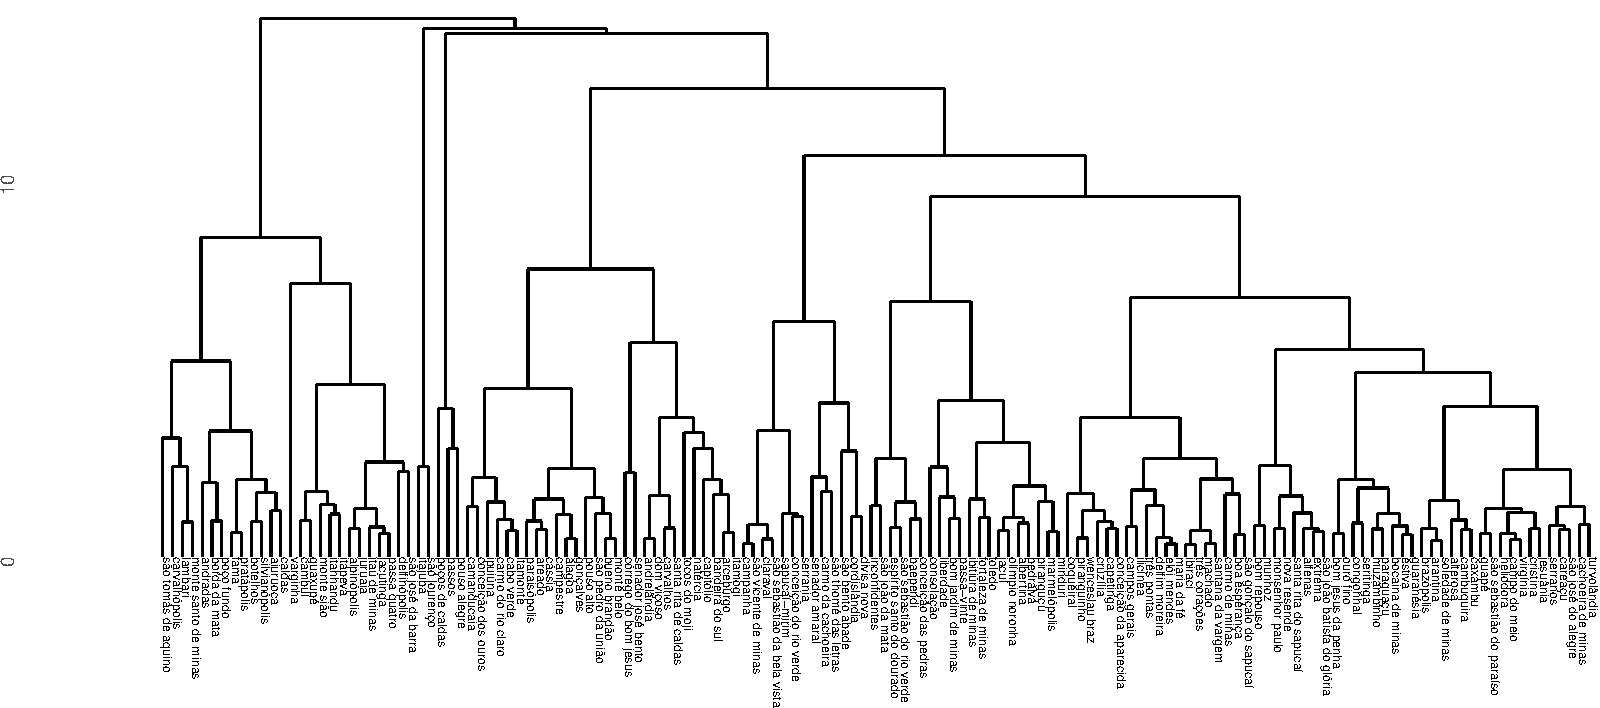
\includegraphics[scale=0.42]{ward_dend_crop}
\end{center}
\caption{Dendrograma pelo método de Ward e distância de Mahalanobis.} \label{wr_maha}
\end{figure}
\FloatBarrier


Com o intuito de propor uma visualização espacial da partição dos dados, a Figura \ref{cps} mostra a dispersão dos municípios em função dos escores dos componentes principais dos grupos obtidos pelo método das $k$-médias. 
 

\begin{figure}[htp!]
\begin{center}
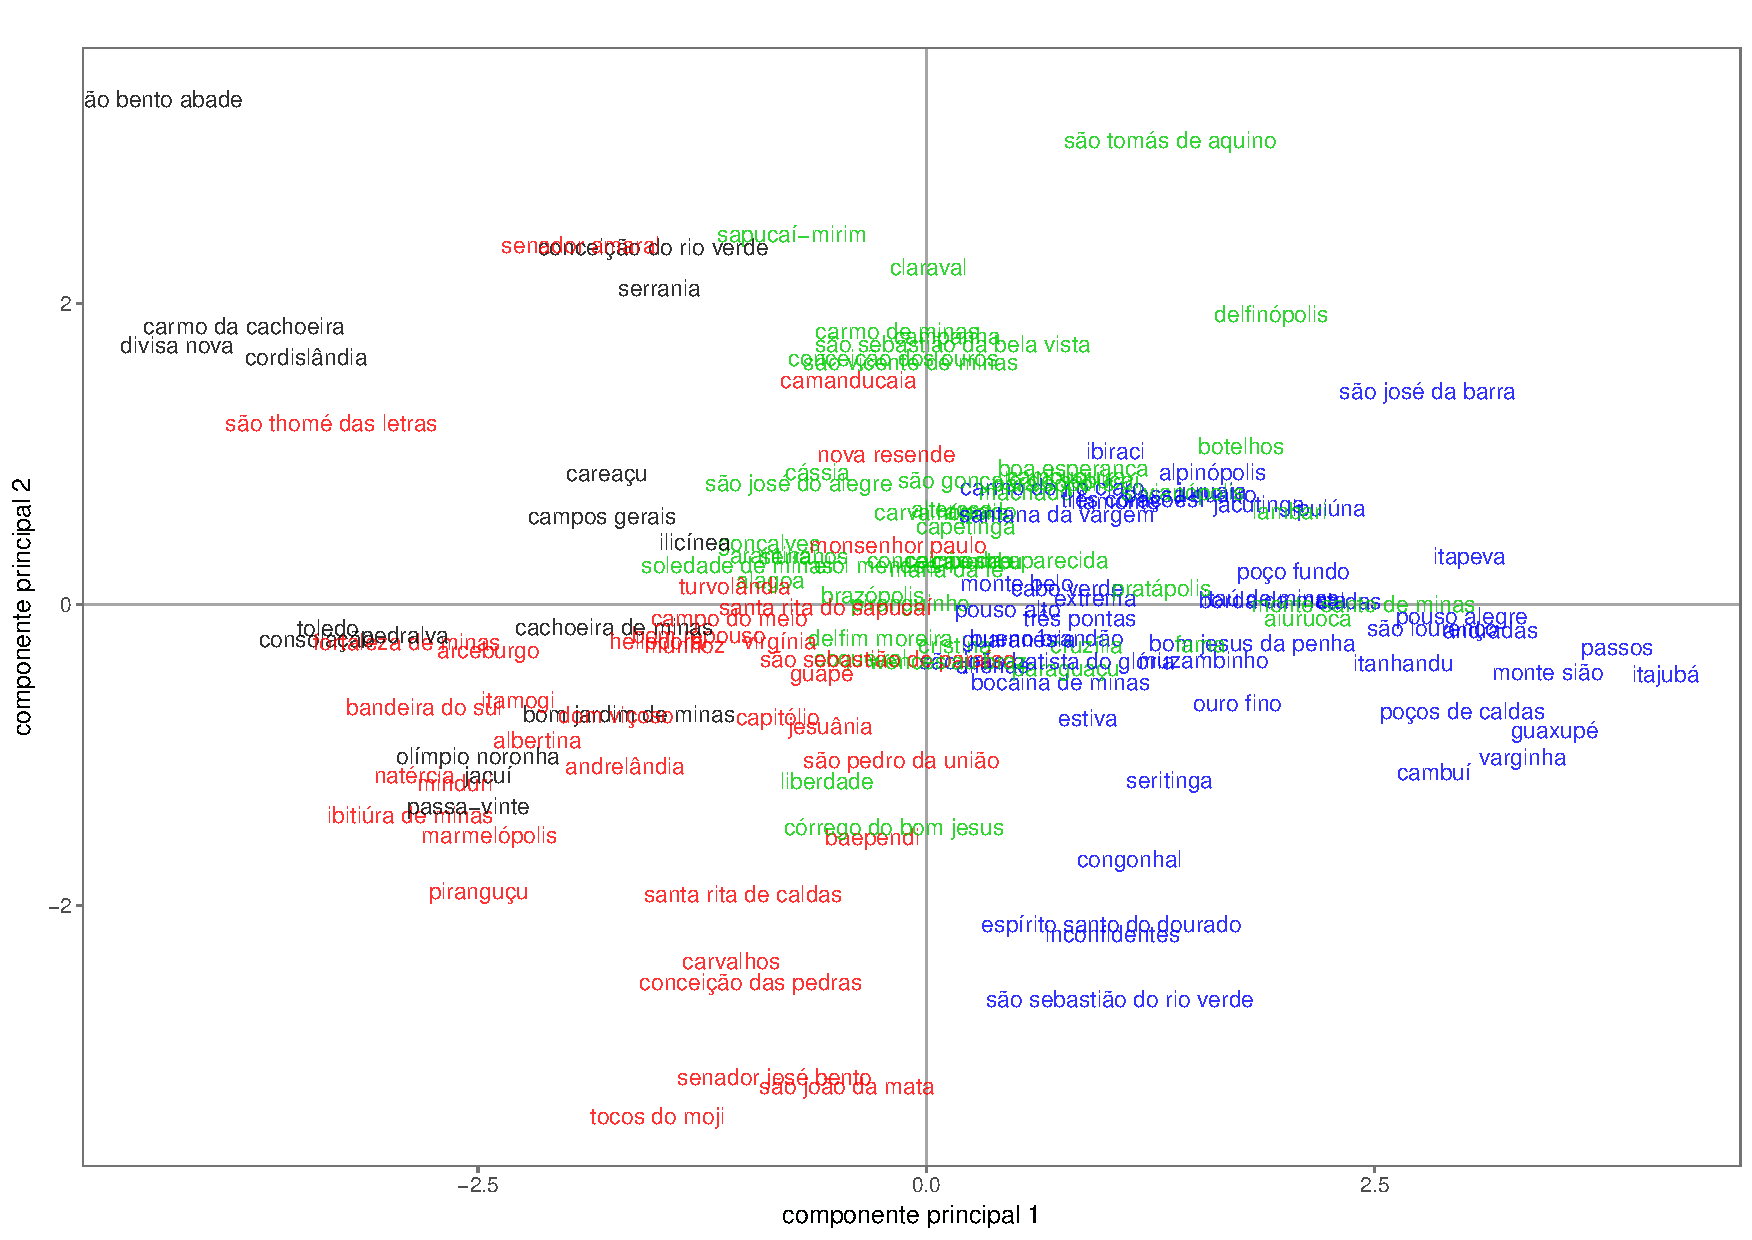
\includegraphics[scale=0.24]{cps_kmeans}
\end{center}
\caption{Dispersão dos municípios em função dos escores dos componentes principais dos quatro grupos obtidos pelo método das $k$-médias.} \label{cps}
\end{figure}
\FloatBarrier

Por esse método os municípios foram divididos em quatro grupos, quanto ao processo de envelhecimento populacional, da seguinte forma: o grupo 1 (G1) é o menor agrupamento, composto por 17 municípios; o grupo 2 (G2) contém 46 municípios; no grupo 3 (G3) estão inseridos 36 municípios e, por último, o grupo 4 (G4) é formado por 47 municípios. A Figura \ref{mapa_grupos} apresenta os quatro grupos no mapa da mesorregião SSM. De forma geral, com exceção do grupo 1, é possível perceber uma certa tendência de municípios vizinhos pertencerem a um mesmo grupo. Contudo, não houve concentração dos municípios de cada grupo em uma única região do mapa. Por isso, ao longo de toda a extensão territorial da mesorregião são encontrados municípios em diferentes estágios do processo de envelhecimento populacional.

%As Tabelas \ref{G1}, \ref{G2}, \ref{G3} e \ref{G4} do Apêndice B apresentam os nomes dos municípios classificados dentro de cada grupo.


\begin{figure}[htp!]
\begin{center}
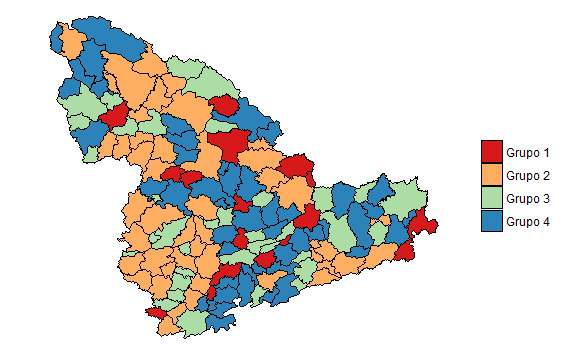
\includegraphics[width=10cm]{mapa}
\end{center}
\caption{Mapa dos municípios da mesorregião Sul/Sudoeste de Minas Gerais classificados em quatro grupos pelo método das $k$-médias.}
\label{mapa_grupos}
\end{figure}
\FloatBarrier

Foram considerados grupos mais envelhecidos aqueles que apresentaram os maiores valores das variáveis espvida e sobre60 e os menores de tft, mort1 e rd. Embora exista um consenso de que quanto maior o valor da t\_env, mais envelhecido é o município, ela não foi decisiva na separação dos grupos. Dois dos quatro grupos se destacaram por possuírem um perfil bem definido, o grupo 1 e o 2 (apresentados nas Tabelas \ref{G1} e \ref{G2}). No G1 estão os municípios menos envelhecidos, ou seja, aqueles que apresentam os piores desempenhos nos indicadores demográficos estudados. Enquanto, no G2 estão os municípios mais avançados no processo de envelhecimento populacional.  

%\begin{table}[!ht]
%\centering
%\caption{Municípios da mesorregião Sul/Sudoeste de Minas Gerais classificados no grupo 1 (G1) pelo método das $k$-médias.}
%\label{G1}
%\[\begin{tabular}{llll}
%\hline
%\multicolumn{4}{c}{Municípios}                                            \\ \hline
%Bom Jardim de Minas & Conceição do Rio Verde & Jacuí           & Serrania \\
%Cachoeira de Minas  & Consolação             & Olímpio Noronha & Toledo   \\
%Campos Gerais       & Cordislândia           & Passa-Vinte     &          \\
%Careaçu             & Divisa Nova            & Pedralva        &          \\
%Carmo da Cachoeira  & Ilicínea               & São Bento Abade &          \\ \hline
%\end{tabular} \]
%\end{table}
%\FloatBarrier

\begin{table}[!ht]
\centering
\caption{Municípios da mesorregião Sul/Sudoeste de Minas Gerais classificados no grupo 1 (G1) pelo método das $k$-médias.}
\label{G1}
\[ \begin{tabular}{lll}
\hline
\multicolumn{3}{c}{municípios}                             \\ \hline
Bom Jardim de Minas    & Consolação      & Passa-Vinte     \\
Cachoeira de Minas     & Cordislândia    & Pedralva        \\
Campos Gerais          & Divisa Nova     & São Bento Abade \\
Careaçu                & Ilicínea        & Serrania        \\
Carmo da Cachoeira     & Jacuí           & Toledo          \\
Conceição do Rio Verde & Olímpio Noronha &                 \\ \hline
\end{tabular} \]
\end{table}
\FloatBarrier



\begin{table}[!ht]
\centering
\caption{Municípios da mesorregião Sul/Sudoeste de Minas Gerais classificados no grupo 2 (G2) pelo método das $k$-médias.}
\label{G2}
\[ \begin{tabular}{lll}
\hline
\multicolumn{3}{c}{municípios}                                         \\ \hline
Alfenas                   & Guaxupé       & Passos                     \\
Alpinópolis               & Ibiraci       & Poço Fundo                 \\
Andradas                  & Inconfidentes & Poços de Caldas            \\
Bocaina de Minas          & Ipuiúna       & Pouso Alegre               \\
Bom Jesus da Penha        & Itajubá       & Pouso Alto                 \\
Borda da Mata             & Itamonte      & Santana da Vargem          \\
Bueno Brandão             & Itanhandu     & São João Batista do Glória \\
Cabo Verde                & Itapeva       & São José da Barra          \\
Caldas                    & Itaú de Minas & São Lourenço               \\
Cambuí                    & Jacutinga     & São Sebastião do Rio Verde \\
Carmo do Rio Claro        & Juruaia       & Seritinga                  \\
Congonhal                 & Monte Belo    & Três Corações              \\
Espírito Santo do Dourado & Monte Sião    & Três Pontas                \\
Estiva                    & Muzambinho    & Varginha                   \\
Extrema                   & Ouro Fino     &                            \\
Guaranésia                & Passa Quatro  &                            \\ \hline
\end{tabular}  \]
\end{table}
\FloatBarrier

Os grupos G3 e G4 (apresentados nas Tabelas \ref{G3} e \ref{G4}, por sua vez, são caracterizados por apresentarem valores intermediários nas variáveis estudadas. O grupo 3 apresenta um comportamento mais próximo do G1 na maior parte das variáveis, ou seja, ele é caracterizado por ser menos envelhecido. Ao mesmo tempo que o G4 possui um comportamento mais próximo do G2 e, portanto, é formado por municípios mais envelhecidos. Com isso, os grupos 2, 4, 3 e 1 representam a ordem dos mais envelhecidos para os menos envelhecidos. 

%Primeiro serão apresentados os resultados dos grupos 1 e 2, em seguida dos demais. 

\begin{table}[!ht]
\centering
\caption{Municípios da mesorregião Sul/Sudoeste de Minas Gerais classificados no grupo 3 (G3) pelo método das $k$-médias.}
\label{G3}
\[\begin{tabular}{lll}
\hline
\multicolumn{3}{c}{municípios}                                       \\ \hline
Albertina            & Fortaleza de Minas & Piranguçu                \\
Andrelândia          & Guapé              & Santa Rita de Caldas     \\
Arceburgo            & Heliodora          & Santa Rita do Sapucaí    \\
Baependi             & Ibitiúra de Minas  & São João da Mata         \\
Bandeira do Sul      & Itamogi            & São Pedro da União       \\
Bom Repouso          & Jesuânia           & São Sebastião do Paraíso \\
Camanducaia          & Marmelópolis       & São Thomé das Letras     \\
Campo do Meio        & Minduri            & Senador Amaral           \\
Capitólio            & Monsenhor Paulo    & Senador José Bento       \\
Carvalhos            & Munhoz             & Tocos do Moji            \\
Conceição das Pedras & Natércia           & Turvolândia              \\
Dom Viçoso           & Nova Resende       & Virgínia                 \\ \hline
\end{tabular}\]
\end{table}
\FloatBarrier


\begin{table}[!ht]
\centering
\caption{Municípios da mesorregião Sul/Sudoeste de Minas Gerais classificados no grupo 4 (G4) pelo método das $k$-médias.}
\label{G4}
\[\begin{tabular}{lll}
\hline
\multicolumn{3}{c}{municípios}                                        \\ \hline
Aiuruoca       & Claraval               & Monte Santo de Minas        \\
Alagoa         & Conceição da Aparecida & Paraguaçu                   \\
Alterosa       & Conceição dos Ouros    & Paraisópolis                \\
Arantina       & Coqueiral              & Piranguinho                 \\
Areado         & Córrego do Bom Jesus   & Pratápolis                  \\
Boa Esperança  & Cristina               & São Gonçalo do Sapucaí      \\
Botelhos       & Cruzília               & São José do Alegre          \\
Brazópolis     & Delfim Moreira         & São Sebastião da Bela Vista \\
Cambuquira     & Delfinópolis           & São Tomás de Aquino         \\
Campanha       & Elói Mendes            & São Vicente de Minas        \\
Campestre      & Fama                   & Sapucaí-Mirim               \\
Capetinga      & Gonçalves              & Serranos                    \\
Carmo de Minas & Lambari                & Silvianópolis               \\
Carvalhópolis  & Liberdade              & Soledade de Minas           \\
Cássia         & Machado                & Wenceslau Braz              \\
Caxambu        & Maria da Fé            &                             \\ \hline
\end{tabular}\]
\end{table}
\FloatBarrier


Para auxiliar na análise dos resultados foram utilizados gráficos \textit{boxplots} apresentados na Figura \ref{box} e algumas medidas estatísticas mostradas na Tabela \ref{medg}. A partir desses resultados foi possível encontrar o perfil demográfico de cada agrupamento resultante. O grupo 1 registrou a menor mediana de espvida (73,56 anos). Além disso, o maior valor do indicador dentro desse grupo foi de 75,01 anos (Conceição do Rio Verde), que ainda está muito abaixo dos outros agrupamentos. A menor espvida do G1 foi de 73,03 anos, experimentada por Divisa Nova, Carmo da Cachoeira e São Bento Abade. Por outro lado, o grupo 2 foi responsável pelos maiores valores de mediana (76,60 anos),  mínimo (75,45 anos) e máximo (78,15 anos). Os municípios de Alfenas e Passos representam os valores de mínimo e máximo do G2, respectivamente. Portanto, um indivíduo de qualquer município do segundo grupo esperava viver, em média, mais anos do que aqueles pertencentes aos demais. Por último, ainda considerando a variável espvida, o G2 apresentou a maior variabilidade nos dados, representada pela diferença entre o terceiro e primeiro quartil. O indicador espvida representa a longevidade do município, nesse sentido quanto menor seu nível de mortalidade, maior será a espvida.

\begin{figure}[htp!]
\begin{center}
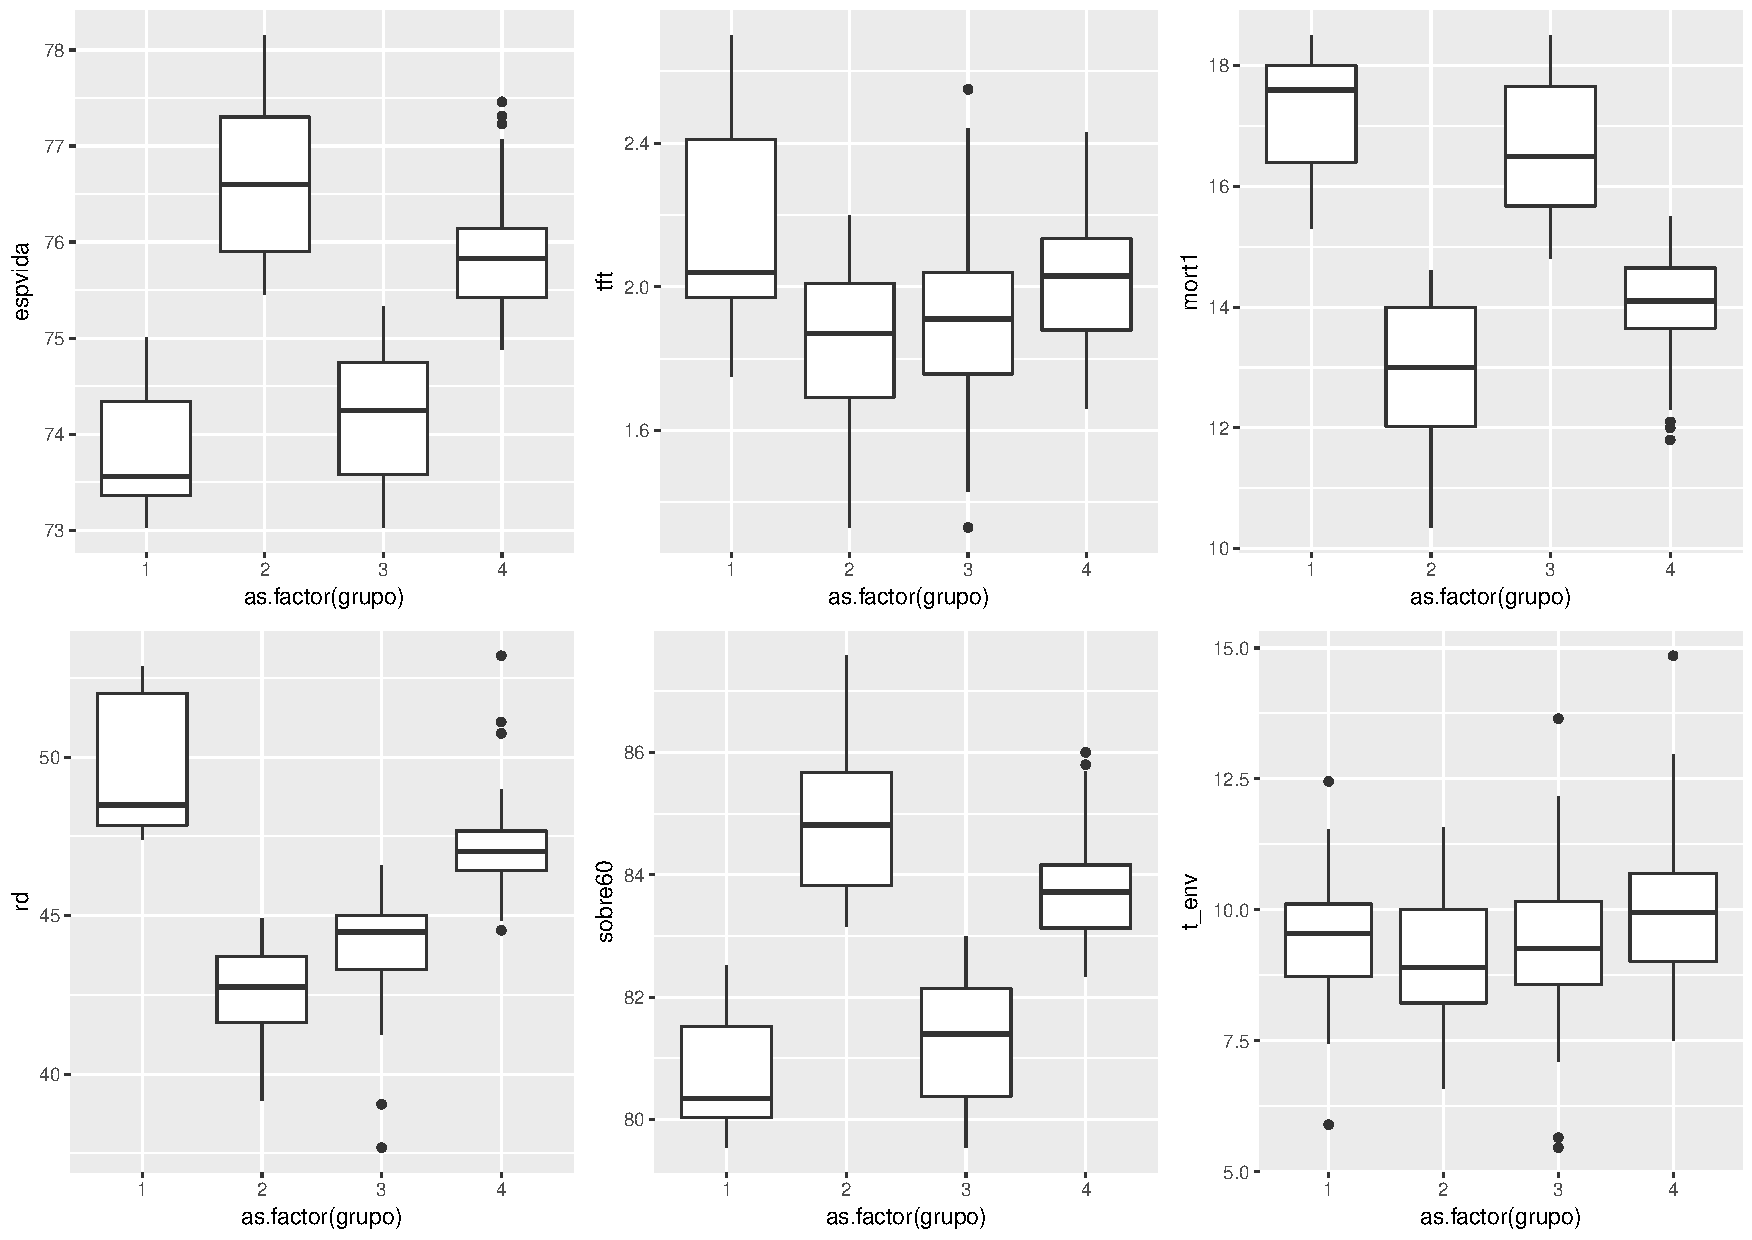
\includegraphics[width=9.75cm]{boxplots1}
\end{center}
\caption{\textit{Boxplots} dos grupos da SSM de acordo com as variáveis: esperança de vida ao nascer (espvida), taxa de fecundidade total (tft), mortalidade infantil (mort1), razão de dependência (rd), probabilidade de sobrevivência até 60 anos (sobre60) e taxa de envelhecimento (t\_env)} \label{box}
\end{figure}
\FloatBarrier

No caso da variável tft, o primeiro grupo apresentou mediana, mínimo e máximo superiores aos outros agrupamentos, o que contribuiu para que ele fosse classificado como o menos envelhecido. Pelo menos 50\% dos municípios experimentaram tft maior que 2,04 filhos por mulher. Além disso, é necessário mencionar que 6 dos 17 municípios do grupo tiveram tft maior que o nível de reposição (2,10 filhos por mulher). O município de Jacuí registrou o menor valor do indicador (1,75 filhos por mulher). Em contrapartida, São Bento Abade foi responsável pela maior tft (2,70 filhos por mulher). Os resultados revelam ainda que o G1 foi o que apresentou maior variabilidade nos dados, considerando essa variável. Sob a perspectiva do grupo 2, o comportamento do nível de fecundidade é muito diferente. O menor nível foi de São Sebastião do Rio Verde (1,33 filhos por mulher) e o maior de Carmo do Rio Claro (2,20 filhos por mulher). Pelo menos metade dos municípios desse grupo possuem uma tft maior que 1,87 filhos por mulher. Além disso, apenas seis dos seus 46 municípios estão acima do nível de reposição e com valores muito próximos dele. Os indicadores desses seis municípios estão compreendidos entre 2,12 e 2,20 filhos por mulher. Quanto menor a tft do município, mais envelhecido ele se torna.


% Please add the following required packages to your document preamble:
% \usepackage{multirow}
\begin{table}[!ht]
\centering
\caption{Resumo estatístico das variáveis demográficas dos grupos obtidos pelo método das $k$-médias.}
\label{medg}
\[ \begin{tabular}{lrrrrrrr}
\hline
\multicolumn{1}{c}{medida} & \multicolumn{1}{c}{grupo} & \multicolumn{1}{c}{espvida} & \multicolumn{1}{c}{tft} & \multicolumn{1}{c}{mort1} & \multicolumn{1}{c}{rd} & \multicolumn{1}{c}{sobre60} & \multicolumn{1}{c}{t\_env} \\ \hline
\multirow{4}{*}{Mediana}    & 1                          & 73,56                        & 2,04                     & 17,60                      & 48,49                   & 80,34                        & 9,55                       \\
                            & 2                          & 76,60                        & 1,87                     & 13,00                      & 42,75                   & 84,81                        & 8,90                       \\
                            & 3                          & 74,25                        & 1,91                     & 16,50                      & 44,49                   & 81,40                        & 9,26                       \\
                            & 4                          & 75,83                        & 2,03                     & 14,10                      & 47,03                   & 83,72                        & 9,95                       \\ \hline
\multirow{4}{*}{CV}         & 1                          & 0,93                         & 13,84                    & 6,53                       & 4,31                    & 1,28                         & 16,23                      \\
                            & 2                          & 0,99                         & 12,04                    & 8,84                       & 3,57                    & 1,31                         & 13,72                      \\
                            & 3                          & 0,94                         & 14,38                    & 6,84                       & 4,25                    & 1,29                         & 17,73                      \\
                            & 4                          & 0,94                         & 9,89                     & 7,32                       & 3,44                    & 1,22                         & 14,86                      \\ \hline
\multirow{4}{*}{Mínimo}     & 1                          & 73,03                        & 1,75                     & 15,30                      & 47,40                   & 79,54                        & 5,90                       \\
                            & 2                          & 75,45                        & 1,33                     & 10,35                      & 39,18                   & 83,16                        & 6,59                       \\
                            & 3                          & 73,03                        & 1,33                     & 14,80                      & 37,68                   & 79,54                        & 5,46                       \\
                            & 4                          & 74,88                        & 1,66                     & 11,80                      & 44,54                   & 82,33                        & 7,51                       \\ \hline
\multirow{4}{*}{Máximo}     & 1                          & 75,01                        & 2,70                     & 18,50                       & 52,86                   & 82,52                        & 12,45                      \\
                            & 2                          & 78,15                        & 2,20                     & 14,60                       & 44,92                   & 87,58                        & 11,57                      \\
                            & 3                          & 75,33                        & 2,55                     & 18,50                       & 46,57                   & 82,99                        & 13,65                      \\
                            & 4                          & 77,46                        & 2,43                     & 15,5                       & 53,20                   & 86,00                        & 14,85                      \\ \hline
\end{tabular} \]
\end{table}
\FloatBarrier

O G1 também apresentou o pior desempenho em relação à variável mort1. Esse comportamento é confirmado pelos altos valores registrados pela mediana (17,60 óbitos por mil nascidos vivos), mínimo (15,30 óbitos por mil nascidos vivos) e máximo (18,50 óbitos por mil nascidos vivos). Como mencionado anteriormente, a longevidade de uma população está associada aos seus níveis de mortalidade. Isso fica evidente ao se observar que o município com a menor mortalidade infantil é o mesmo que apresentou a maior espvida (Conceição do Rio Verde). Da mesma forma, os municípios Divisa Nova, Carmo da Cachoeira e São Bento Abade são responsáveis pelos maiores níveis de mortalidade infantil e menores espvida. Por outro lado, o segundo grupo registrou mediana, mínimo e máximo inferiores aos demais. Pelo menos metade dos municípios apresentam mortalidade infantil inferior à 13 óbitos por mil nascidos vivos. O município de Passos experimentou a menor mortalidade infantil (10,35 óbitos por mil nascidos vivos) e Alfenas a maior (14,60 óbitos por mil nascidos vivos).

No que diz respeito ao indicador rdt, no primeiro grupo foram observados os maiores valores de mediana, (48,49\%), mínimo (47,40\%) e máximo (52,86\%). Os municípios de Cachoeira de Minas e Divisa Nova experimentaram o menor e maior valores do indicador, respectivamente. Deve-se lembrar que, à medida que a população avança no processo de envelhecimento, primeiro é esperado uma redução da rdt. Logo, no ano estudado, os valores altos da variável não indicam um bom desempenho. Isso reafirma a desvantagem do G1 em relação aos outros. Por outro lado, o segundo grupo teve mediana, mínimo e máximo inferiores aos demais. Pelo menos 50\% dos municípios desse grupo apresentaram rdt menor que 42,75\%, limitado por um valor mínimo de 39,18\% (Varginha) e máximo de 44,92\% (Passos).

Em relação à variável sobre60, dentre os municípios alocados no primeiro grupo, estão os que registraram o menor valor da mesorregião SSM. Os resultados apontam que Divisa Nova, São Bento Abade e Carmo da Cachoeira representam o mínimo de 79,54\%. Esse agrupamento também registra valores de mediana (80,34\%) e máximo (82,52\%) inferiores aos outros três agrupamentos. Do mesmo modo, o G2 mais uma vez se destacou por um comportamento melhor que os demais. Pelo menos 50\% dos municípios desse grupo experimentam sobre60 maiores que 84,31\%. O menor valor foi experimentando por Alfenas  (83,16\%) e o maior por Itajubá (87,58\%).

E, finalmente, a análise da variável t\_env mostrou que o primeiro grupo apresentou mediana de 9,55\%. Essa foi a única variável desse agrupamento com pontos discrepantes. Os municípios de Consolação (12,45\%) e São Bento Abade (5,90\%) foram esses \textit{outliers}. No segundo grupo, a mediana foi de 8,90\%. O município de São José da Barra foi o responsável pelo menor valor do indicador (6,59\%) e Poços de Caldas o maior (11,57\%). O terceiro e quarto agrupamento serão analisados a seguir, contudo já é possível adiantar que as estatísticas dessa variável pouco se diferenciaram entre os grupos. Em razão disso, mesmo usada como critério para estudar o envelhecimento populacional, essa variável pouco contribuiu para entender a classificação dos municípios entre os grupos. 

No que diz respeito ao terceiro e quarto grupos, observou-se que os municípios classificados neles possuem um comportamento intermediário nos indicadores considerados. Em relação às variáveis espvida, mort1 e sobre60, o G4 teve um comportamento semelhante G2. Ao passo que o G3 registrou valores mais aproximados do G1, ou seja, caracterizando um grupo menos envelhecido. Em pelo menos 50\% dos municípios do G3, os indivíduos esperavam viver em média mais do que 74,25 anos, enquanto no G4 esse valor foi de 75,83 anos. Além disso, esses valores foram limitados por um máximo de 75,33 anos (São Sebastião do Paraíso) no terceiro grupo e 77,46 anos no quarto (Monte Santo de Minas e São Tomás de Aquino). O valor mínimo foi de 73,03 anos no terceiro agrupamento (São Thomé das Letras) e 74,88 anos no quarto (Soledade de Minas). O G4 além de ser caracterizado pela menor variação nos dados, é o único que apresenta pontos discrepantes, sendo eles São Tomás de Aquino e Monte Santo de Minas (77,46 anos), Delfinópolis (77,31 anos), Lambari e Aiuruoca (77,23 anos).

Quanto à variável mort1, os resultados indicam que o quarto grupo foi o que apresentou menor variabilidade. Além do mais, também foram identificados pontos discrepantes nesse agrupamento, sendo eles São Tomás de Aquino e Monte Santos de Minas (11,80 óbitos por mil nascidos vivos), Delfinópolis (12 óbitos por mil nascidos vivos), Lambari e Aiuruoca (12,10 óbitos por mil nascidos vivos). A mediana de 14,10 óbitos por mil nascidos vivos foi menor que do terceiro grupo (16,50 óbitos por mil nascidos vivos). Os resultados de mínimo e máximo reafirmam o melhor desempenho do G4 comparado ao G3. O limite inferior do quarto agrupamento (11,80 óbitos por mil nascidos vivos) é menor que do terceiro (14,80 óbitos por mil nascidos vivos). Eles são representados pelos municípios de Monte Santo de Minas e São Tomás de aquino (grupo 4) e São Sebastião do Paraíso (grupo 3). Do mesmo modo, o limite superior é menor para o quarto agrupamento (15,50 óbitos por mil nascidos vivos) do que para o terceiro (18,50 óbitos por mil nascidos vivos. Os municípios de Soledade de Minas e São Thomé das Letras são os responsáveis por esses indicadores, respectivamente. 

No caso da variável sobre60, o quarto grupo foi o único com pontos discrepantes, sendo eles São Tomás de Aquino e Monte Santo de Minas (86\%) e Delfinópolis (85,80\%). Quando comparado aos grupos 1 e 3, é possível observar que o quarto agrupamento apresentou melhor desempenho na sobre60. O ponto de mínimo desse grupo foi de 82,52\% (Liberdade) e o de máximo foi de 86\% (São Tomás de Aquino e Monte Santo de Minas). Pelo menos 50\% dos municípios pertencentes a esse agrupamento apresentaram sobre60 maior que 83,72\%. Por fim, o G3 registrou valores de mínimo, máximo e mediana inferiores aos grupos 2 e 4. Isso também contribuiu para esse agrupamento ser classificado como menos envelhecido, assim com o primeiro. A mediana foi de 81,40\% com valores limitados por um mínimo de 79,54\% (São Thomé das Letras) e máximo de 82,99\% (Nova Resende). 

Apesar das estatísticas da t\_env serem muito parecidas entre os agrupamentos e, em função disso, contribuírem menos para a divisão dos grupos, o quarto grupo parece apresentar um comportamento melhor que o terceiro. A mediana desse agrupamento foi de 9,95\%, ao passo que do terceiro foi de 9,26\%. O menor valor do indicador registrado no G4 foi de 7,51\% (Carmo de Minas) e o maior, um ponto discrepante no conjunto de observações, foi de 14,85\% (Córrego do Bom Jesus). O município Senador Amaral foi responsável pelo valor mínimo no G3 (5,46\%) e Senador José Bento pelo máximo (13,65\%). Os dois municípios também são pontos discrepantes, assim como São Thomé das Letras (5,65\%).

Em contrapartida, quando se analisam os agrupamentos em relação às variáveis tft e rdt, verifica-se que o grupo 3 apresentou melhores resultados que o 4. Pelo menos 50\% dos municípios do terceiro agrupamento experimentaram tft abaixo de 1,91 filhos por mulher, enquanto no quarto agrupamento esse valor alcançou 2,03 filhos por mulher. Os valores de mínimo e máximo do G3 são dois pontos discrepantes, sendo eles Senador Amaral (2,55 filhos por mulher) e São João da Mata (1,33 filhos por mulher). No G4, os municípios de Liberdade e São Tomás de Aquino representam o mínimo (1,66 filhos por mulher) e máximo (2,43 filhos por mulher), respectivamente. Por último, no que diz respeito à rdt, os municípios classificados no G3 apresentam valores inferiores aos do G4. O mínimo do terceiro agrupamento foi de 37,68\% (Tocos do Moji), enquanto do quarto é de 44,54\% (Campestre). O município de Turvolândia registrou o valor máximo (46,57\%) no terceiro grupo, ao passo que São Tomás de Aquino (53,20\%) no quarto grupo.

Para avaliar a homogeneidade interna dos grupos foi usado o coeficiente de variação (CV) de cada variável. Quanto menor seu valor, mais homogêneo é considerado o agrupamento em relação àquela variável. De forma geral, os resultados mostram que todos os grupos apresentaram valores baixos em relação a todas as variáveis, o que aponta para homogeneidade interna. A variável espvida foi responsável pelos menores valores de CV, enquanto as variáveis t\_env e tft pelos maiores.
Por último, as variáveis população (pop) e rendimento médio dos ocupados (renocup) foram selecionadas para auxiliar na caracterização dos grupos obtidos. A Figura \ref{box22} mostra os \textit{boxplots} dos grupos de acordo com essas variáveis e a Tabela \ref{table1} apresenta a mediana, o CV, o mínimo e máximo dos grupos para cada uma dessas variáveis.

\begin{figure}[htp!]
\begin{center}
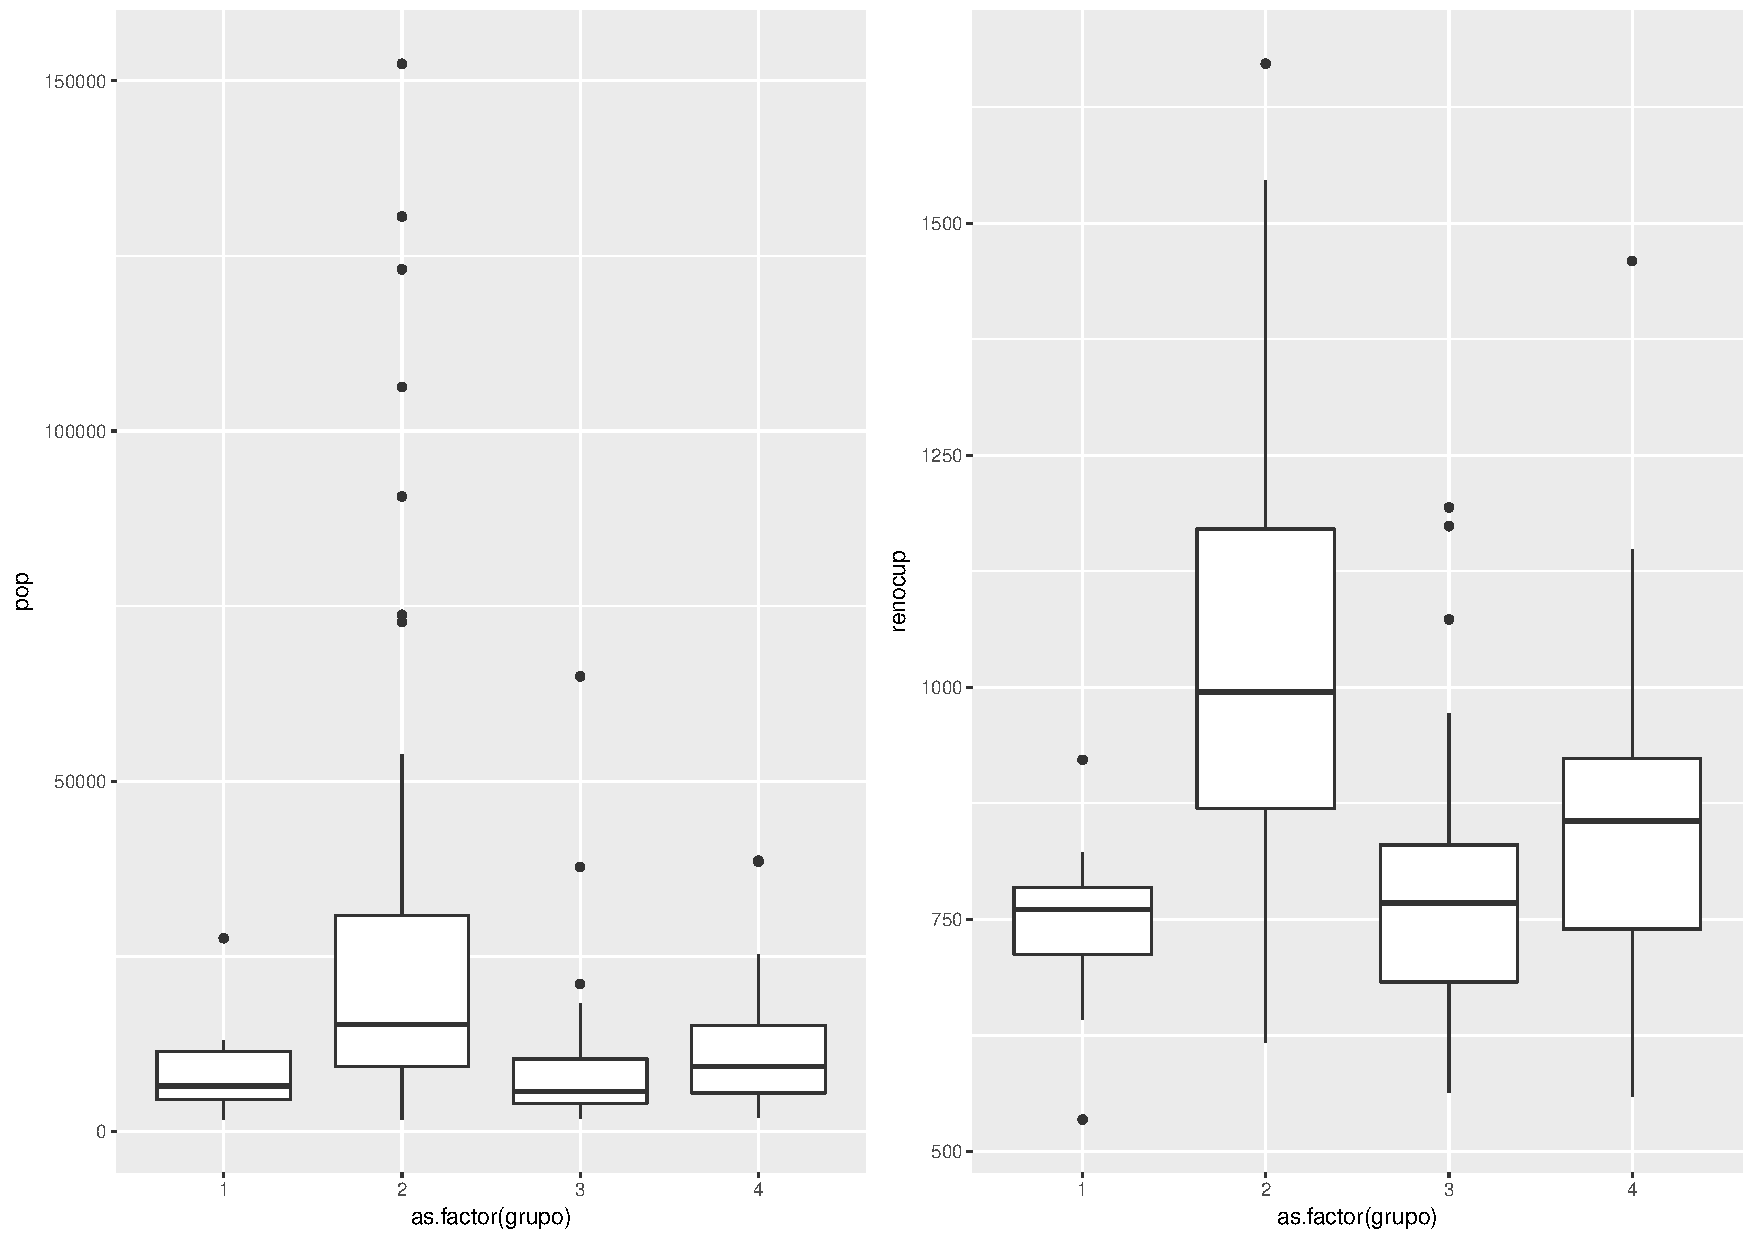
\includegraphics[width=10cm]{boxplots2}
\end{center}
\caption{\textit{Boxplots} dos grupos da SSM de acordo com as variáveis população (pop) e rendimento médio dos ocupados (renocup).} \label{box22}
\end{figure}
\FloatBarrier

A variável pop foi escolhida com o intuito de conhecer o tamanho da população dos municípios dentro de cada grupo. Os resultados mostram que pelo menos 50\% dos municípios do G1 (grupo menos envelhecido) possuem uma população menor que 6.501 habitantes, com um mínimo de 1.727 (Consolação) e máximo de 27.600 (Campos Gerais), que é um ponto discrepante no conjunto de dados. Portanto, o que se observa é um grupo composto por pequenos municípios. No grupo mais envelhecido (G2), por sua vez, estão inseridos grande parte dos municípios maiores como Poços de Caldas, Pouso Alegre, Varginha e Passos, que representam os únicos municípios com mais de 100.000 pessoas da mesorregião. No entanto, nesse grupo também estão inseridos municípios que estão entre os menores da SSM em termos de população, como por exemplo, São Sebastião do Rio Verde (2.107 habitantes), Bom Jesus da Penha (3.842 habitantes), Espírito Santo do Dourado (4.426 habitantes), entre outros. Pelo menos 50\% dos municípios do segundo grupo apresentam população menor que 15.263 habitantes, com um mínimo de 1.789 (Seritinga) e máximo de 152.435 (Poços de Caldas). Além disso, esse é o grupo que possui maior variabilidade nos dados e também o maior número de \textit{outliers}, como pode ser obervado pelo \textit{boxplot}.

% Please add the following required packages to your document preamble:
% \usepackage{multirow}
\begin{table}[!ht]
\centering
\caption{Resumo estatístico das variáveis população (pop) e rendimento médio dos ocupados (renocup) dos grupos obtidos pelo método das $k$-médias.}
\label{table1}
\[ \begin{tabular}{lrrr}
\hline
\multicolumn{1}{c}{medida} & \multicolumn{1}{c}{grupo} & \multicolumn{1}{c}{pop} & \multicolumn{1}{c}{renocup} \\ \hline
\multirow{4}{*}{Mediana}    & 1                          & 6.501                    & 760,59                      \\
                            & 2                          & 15.263                   & 995,09                      \\
                            & 3                          & 5.729                    & 767,55                      \\
                            & 4                          & 9.289                    & 855,90                      \\ \hline
\multirow{4}{*}{CV}         & 1                          & 74,82                    & 11,72                       \\
                            & 2                          & 120,16                   & 23,32                       \\
                            & 3                          & 120,22                   & 18,97                       \\
                            & 4                          & 73,18                    & 17,99                       \\ \hline
\multirow{4}{*}{Mínimo}     & 1                          & 1.727                    & 534,51                      \\
                            & 2                          & 1789                     & 617,29                      \\
                            & 3                          & 1868                     & 563,11                      \\
                            & 4                          & 1995                     & 558,92                      \\ \hline
\multirow{4}{*}{Máximo}     & 1                          & 27.600                   & 921,96                      \\
                            & 2                          & 152.435                  & 1671,92                     \\
                            & 3                          & 64.980                   & 1193,90                     \\
                            & 4                          & 38.688                   & 1459,40                     \\ \hline
\end{tabular} \]
\end{table}
\FloatBarrier


A migração interna, que corresponde aquela que ocorre dentro de um mesmo território, ou seja, entre regiões, estados e municípios do país, contribui pra explicar a classificação de pequenos municípios em um grupo mais avançado no processo de envelhecimento populacional. De forma geral, o que se observa é uma migração de jovens para os municípios maiores e mais desenvolvidos, em busca de trabalho e renda (CAMPOS; BARBIERI, 2013). Diante disso, a migração interna exerce papel importante na definição da estrutura etária da população. Isso ocorre porque a mudança dos jovens para os grandes centros contribui para intensificar o processo de envelhecimento populacional nos municípios menores (WONG; CARVALHO, 2006). A saída deles, além de aumentar a proporção de idosos na população, também contribui pra reduzir o nível de fecundidade da população. 

Por outro lado, a estrutura etária das cidades maiores também se torna, em parte, reflexo da imigração dos jovens. Isso ajuda a explicar a razão de os municípios de Pouso Alegre, Varginha e Três Corações estarem entre aqueles que experimentam as menores proporções de pessoas com 65 anos (t\_env) da mesorregião SSM. Os jovens migrantes que ingressam nesses municípios contribuem, em um primeiro momento, para aumentar o denominador da taxa (população total) e, portanto, reduzir a proporção de idosos. Essa análise sobre a variável t\_env é interessante, pois ela mostra como uma visão geral sobre as variáveis separadas pode comprometer a realidade dos municípios. Caso o envelhecimento da população fosse estudado usando apenas a proporção de idosos com mais de 65 anos de idade, Varginha que possui t\_env de 7,17\% seria considerada menos envelhecida que Consolação (12,45\%), por exemplo. Entretanto, considerando as demais variáveis demográficas na análise multivariada, Varginha foi classificada no grupo mais envelhecido e Consolação no menos envelhecido. 

Campos e Barbieri (2013) também discutem o processo de migração dos idosos, os autores ressaltam que é possível observar duas direções nos fluxos migratórios desse grupo. A primeira refere-se a idosos que migram de municípios maiores para os menores, em busca de segurança e qualidade de vida. A segunda diz respeito aos idosos de cidades menores que migram para cidades maiores para acompanhar familiares e/ou na tentativa de obter melhor assistência à saude. Entretanto, a migração dos jovens é muito mais expressiva e exerce um peso muito maior para o envelhecimento da população do município de origem. 

No que diz respeito aos demais grupos, o terceiro (G3) registrou mediana de 5.729 habitantes, mínimo de 1.868 (Senador José Bento) e máximo de 64.980 (São Sebastião do Paraíso), que representa um \textit{outlier}. Esse foi o agrupamento com a menor variabilidade nos dados. O G4 apresentou mediana de 9.289 habitantes, Serranos é o menor município desse grupo, com 1.995 habitantes, enquanto Machado é o maior (38.688). Além disso, os grupos não parecem tão homogêneos em relação à variável pop, principalmente os grupos 2 e 3 que registraram um alto coeficiente de variação.

A variável rendimento médio dos ocupados, que representa em reais a média dos rendimentos de todos os trabalhos das pessoas ocupadas de 18 anos ou mais de idade, também foi analisada em cada grupo obtido. Berquó e Cavenaghi (2006) mostram a contínua redução do declínio da taxa de fecundidade total no Brasil e os diferenciais produzidos nesse processo, através das variáveis educação e renda. Ainda de acordo com as autoras, as mulheres com baixo rendimento domiciliar e escolaridade apresentavam maiores níveis de fecundidade do que aquelas em situação melhor. Essa associação negativa da renda e da escolaridade com o nível de fecundidade foi estudada considerando uma amostra de mulheres em idade reprodutiva (15 a 49 anos) e, especificamente, as variáveis rendimento domiciliar \textit{per capita} e diferentes faixas de anos de estudo. Dada a dificuldade de obter e caracterizar os grupos em relação à escolaridade das mulheres, foi escolhida apenas uma variável relacionada à renda.

Em linhas gerais, foi observado que o grupo mais envelhecido (G2) apresentou melhor desempenho sobre a variável renocup e também maior variabilidade nos dados, como pode ser visto pelo \textit{boxplot}. Em pelo menos 50\% dos municípios desse agrupamento o rendimento médio dos ocupados é maior que R\$ 995,09, Juruaia foi o município responsável pelo maior rendimento médio dos ocupados (R\$ 1.671,96) e Pedralva pelo menor (R\$ 617,29). Por outro lado, a mediana do G1 (menos envelhecido) foi de R\$ 760,59, o mínimo de R\$ 534,51 (Consolação) e máximo de R\$ 921,96, os resultados revelam que nesse grupo são registradas as menores estatísticas relacionadas ao renocup. Os grupos 3 e 4 apresentaram comportamento intermediário, no entanto o G4 registrou melhor desempenho que o G3 em relação a essa variável. As medianas nesses grupos foram de R\$ 767,55 (G3) e R\$ 855,90 (G4). Os municípios de Senador José Bento e Alagoa foram responsáveis pelos menores valores da variável renocup (R\$ 563,11 e R\$ 558,92) nos grupos 3 e 4, respectivamente. Por outro lado, Camanducaia e Caxambu registraram os maiores valores (R\$ 1.193,90 e R\$ 1.459,40) nesses mesmos agrupamentos. Portanto, comparando os quatro grupos em relação à variável renda foi observado que, de forma geral, os municípios dos grupos mais envelhecidos registram um rendimento médio dos ocupados maior que aqueles pertecentes aos grupos menos envelhecidos.

Para avaliar a homogeneidade interna dos grupos em relação às variáveis pop e renocup foram calculados seus coeficientes de variação. Os resultados mostram que as duas variáveis registraram valores um pouco mais elevados que aquelas utilizadas na análise multivariada. No entanto, o que mais chama atenção são os altos valores da variável pop, o que indica que os grupos são pouco homogêneos em relação ao tamanho da população, ou seja, os grupos são formados por municípios com tamanhos populacionais muito diferentes.

	
	%Conclusões (se houverem)
	\section*{Conclusões}
	
Na literatura há diversos trabalhos que estudam o processo de transição demográfica e o consequente envelhecimento populacional. De forma geral, essas e outras variáveis são utilizadas nesses estudos, dentre elas: idade mediana, índice de envelhecimento, taxa bruta de natalidade, taxa bruta de mortalidade e taxa de crescimento anual (VASCONCELOS; GOMES. 2012; LUTZ; SANDERSON; SCHERBOV, 2008; CARVALHO; WONG, 2008). Neste trabalho, para garantir a qualidade e comparabilidade dos dados, foram utilizadas apenas as variáveis demográficas disponíveis no Atlas Brasil.
	
A análise simultânea das diferentes variáveis permitiu uma avaliação muito mais ampla do processo de envelhecimento populacional na mesorregião SSM. No entanto, esse trabalho possui limitações quanto às variáveis e ao método de agrupamento. Para garantir a qualidade e comparabilidade dos dados foram usadas apenas variáveis demográficas disponíveis no Atlas do Desenvolvimento Humano (construído a partir dos censos demográficos do IBGE). Entretanto, o uso de indicadores como a idade mediana, o índice de envelhecimento, entre outros indicadores demográficos e socioeconômicos, poderia fornecer mais informações e até mesmo organizar os municípios em grupos diferentes. Em relação aos métodos de agrupamento, de forma geral eles são imprecisos e a formação dos grupos não é óbvia. A seleção de outros métodos e medidas de distância poderiam resultar em diferentes agrupamentos. Entretanto, como não há uma classificação evidente, utilizou-se o método das $k$-médias, que demonstra um desempenho superior aos métodos
hierárquicos (MOOI; SARSTEDT, 2010). Além disso, é importante ressaltar que os grupos foram considerados mais envelhecidos ou menos envelhecidos entre si com base na comparação do desempenho das variáveis em cada um deles. Contudo, o quão envelhecido cada grupo está frente ao processo de transição demográfica não foi objeto de estudo desse trabalho.

Um tema recorrente para a teoria da transição demográfica diz respeito ao seu momento de início, magnitudade e velocidade, que são diferentes para os diversos países e regiões do mundo. Nesse sentido, eventualmente todos os municípios do Brasil passariam pela transição demográfica e o consequente envelhecimento da população, contudo, não de maneira homogênea. Isso fica nítido com a classificação dos municípios da mesorregião Sul/Sudoeste de Minas Gerais em mais de um agrupamento, representando os diferentes estágios no processo de envelhecimento populacional. O método das $k$-médias propôs uma divisão dos municípios em quatro grupos: o primeiro (G1) constituído por municípios menos envelhecidos, o segundo grupo (G2) formado por municípios que se encontram em um estágio mais avançado do processo de envelhecimento da população e, por último, os grupos G3 e G4 que assumiram posições intermediárias entre os dois primeiros (G3 menos envelhecido que o G4). Aproximadamente 64\% dos municípios foram classificados nos grupos considerados mais envelhecidos (G2 e G4), o que corresponde a 93 dos 146 municípios. 

Esses resultados podem servir como subsídios para os formuladores de políticas públicas, pois diferentes dinâmicas populacionais demandam políticas públicas específicas para cada grupo de municípios. Isso acontece porque as demandas por políticas públicas acabam sendo impostas pela estrutura etária do município. Um grupo de municípios menos envelhecido possivelmente demandará mais recursos direcionados às crianças e à população economicamente ativa. Portanto, é razoável supor que maior atenção seja dada à educação e mercado de trabalho, por exemplo. Por outro lado, os municípios mais envelhecidos precisam se dedicar mais à assistência para a população idosa tanto no âmbito da saúde, como no de infraestrutura, para que seja capaz de atender às necessidades de um envelhecimento ativo e saudável (WONG; CARVALHO, 2006). Diante disso é necessário que a transição da estrutura etária seja considerada para a alocação eficiente de recursos destinados à população (BRITO, 2007).

	\medskip
	
	
	
% equa��o (se houver)
%	\begin{equation}\label{equ:chave}
%	\mbox{Edite a equação}
%	\end{equation}
	
	% figura (se houver)
%	\begin{figure}[htp!]
%		\begin{center}
%			Insira a figura
%		\end{center}
%		\caption{Título da figura.} \label{fig:chave}
%	\end{figure}
	
	% Tabela (se houver)
%	\begin{table}
%		\caption{Título da tabela}\label{tab:chave}
%		\[ \begin{tabular} {lrcrrrc}
%		Edite a tabela
%		\end{tabular} \]
%	\end{table}
	

	%Agradecimentos (se houverem)
%	\section{Agradecimentos}
%	Digite os agradecimentos
%	\medskip
	
	\bigskip
	\noindent{SOUZA, L. G.; RAMOS, P. de S.; FRIAS, L. T. G. de. Population ageing in the cities of South/Southwest of Minas Gerais: cluster analysis. \textit{Rev. Bras. Biom.,} Lavras, v.xx, n.x, p.xx-xx, 20xx.}
	\medskip
	
	\begin{abstract}
		The aim of the present study was to classify the cities which is located in the South/Southwest mesoregion of Minas Gerais about population ageing. Specifically identifying the groups of cities that are more and less advanced in the process of population ageing. The variables selected for the study were: life expectancy at birth, total fertility rate, infant mortality, mortality up to 5 years of age, dependency ratio, probability of survival up to 40 years, probability of survival up to 60 years and ageing rate. These data come from the IBGE Demographic Census of 2010, consulted through the Atlas of Human Development in Brazil. First we used the Ward method to define the number of groups, while the initial centroids were randomly selected. Next, the non-hierarchical method of $k$-means was applied to identify groups of cities with similar characteristics. The results point to the classification of cities in four groups, in relation to the process of population aging.
		
	\end{abstract}
	
	\begin{keyword}
  Cluster analysis; classification; demographic transition
  	\end{keyword}
	
	
	\begin{thebibliography}{}
		
		\bibitem[]{}
		
		% Siga os exemplos a seguir:
		
		%Livro
		
		BERQUÓ, E.; CAVENAGHI, S. Fecundidade em declínio:  breve nota sobre a redução no número médio de filhos por mulher no brasil. \textit{Novos Estudos - CEBRAP}, São Paulo, n. 74, p.11–15, 2006.
			
		BLASHFIELD, R. K. Mixture model tests of cluster analysis: Accuracy of four agglomerative hierarchical methods. \textit{Psychological Bulletin}, v. 83, n. 3, p. 377-388, 1976.
		
		BRITO, F. A transição demográfica no brasil: as possibilidades e os desafios para a economia ea sociedade. \textit{Texto para discussão}, Cedeplar/UFMG, Belo Horizonte, n. 318, p. 28, 2007.
		
		CAMARANO, A. A. O. \textit{Novo regime demográfico: uma nova relação entre população e desenvolvimento?}. Rio de Janeiro: Instituto de Pesquisa Econômica Aplicada (Ipea), 2014. 658 p.
		
		CAMPOS, M. B. de; BARBIERI, A. F. Considerações teóricas sobre as migrações de idosos. \textit{Revista Brasileira de Estudos da População}, São Paulo, v. 30, p. 69–84, 2013.
		
		CARVALHO, J. A. M. d.; GARCIA, R. A. O envelhecimento da populaçäo brasileira:  um enfoque demográfico. \textit{Cad. saúde pública}, Rio de Janeiro, v. 19, n. 3, p. 725–733, 2003.
		
		CARVALHO, J. A. M. d.; WONG, L. R. A transição da estrutura etária da população brasileirana primeira metade do século XXI. \textit{Cadernos de Saúde Pública}, Rio de Janeiro, v. 24, n. 3, p.597–605, 2008.
		
		DOBRIANSKY, P. J.; SUZMAN, R. M.; HODES, R. J. Why population aging matters: A global perspective. \textit{National Institute on Aging, National Institutes of Health, US Department of Health and Human Services, US Department of State}, 2007.
		
		EVERITT, B.; HOTHORN, T. \textit{An introduction to applied multivariate analysis with R}. New York: Springer-Verlag, 2011.
		
		EVERITT, B. S. et al. \textit{Cluster analysis}. 5. ed. United Kingdom: John Wiley and Sons, 2011
		
		FERREIRA, D. F. \textit{Estatística multivariada}. 2. ed. Lavras: Ed. UFLA, 2011. 675 p.
		
		HAIR, J. F.  \textit{Análise multivariada de dados}. 6. ed. Porto Alegre: Bookman, 2009. 688 p.
		
		LATTIN, J.; CARROLL, J. D.; GREEN, P. E. \textit{Análise de Dados Multivariados.} São Paulo: Cengage Learning, 2011. 455 p.
		
		LIMA-COSTA, M. F.; VERAS, R. Saúde pública e envelhecimento. \textit{Cadernos de Saúde Pública}, Rio de Janeiro, v. 19, n. 3, p. 700–701, 2003.
		
		LEE, R. The demographic transition: three centuries of fundamental change. \textit{The journal ofeconomic perspectives}, v. 17, n. 4, p. 167–190, 2003.
		
		LUTZ, W.; SANDERSON, W.; SCHERBOV, S. The coming acceleration of global populationageing. \textit{Nature}, v. 451, n. 7179, p. 716–719, 2008.
		
		MOOI, E.;  SARSTEDT, M. \textit{A Concise Guide to Market Research}. Germany: Springer-Verlag Berlin Heidelberg, 2011. 308 p.
		
		MINGOTI, S. A. \textit{Análise de dados através de métodos de estatística multivariada: uma abordagem aplicada}. Belo Horizonte: Editora UFMG, 2005. 297 p.
		
		PAIVA, P. d. T. A.; WAJNMAN, S. Das causas às consequências econômicas da transição demográfica no brasil. \textit{Revista Brasileira de Estudos Populacionais}, São Paulo, v. 22, n. 2, p.13–15, 2005.
		
		PENA, J. M.;  LOZANO, J. A.;  LARRANAGA, P. An empirical comparison of fourinitialization methods for the k-means algorithm. \textit{Pattern recognition letters}, San Sebastián, v. 20, n. 10, p. 1027–1040, 1999.
		
		R Core Team. \textit{R: A Language and Environment for Statistical Computing}. Vienna, Austria, 2016. Disponível em: https://www.R-project.org/.
		
		RStudio Team. \textit{RStudio: Integrated Development Environment for R}. Boston, MA, 2016. Disponível em: http://www.rstudio.com/.
		
		VASCONCELOS, A. M. N.; GOMES, M. M. F. Transição demográfica:  a experiência brasileira. \textit{Epidemiologia e Serviços de Saúde}, Brasília, v. 21, n. 4, p. 539–548, 2012.
		
		WONG, L. L. R.; CARVALHO, J. A. O rápido processo de envelhecimento populacional do brasil: sérios desafios para as políticas públicas. \textit{Revista Brasileira de Estudos de População}, São Paulo, v. 23, n. 1, p. 5–26, 2006.
		
	%	McCULLACH, P.; NEDER, J. A. \textit{Generalized linear models}.
	%	2.ed. London: Chapman and Hall, 1989. 511p.		
		
		%Cap�tulo de Livro,
	%	ARNOLD, B. C. Multivariate logistic distributions. In: BALAKRISHNAN,
	%	N. (Ed.). \textit{Handbook of the logistic distribution. New York:
	%		Marcel Dekker}, 1992. p.237-261. (Statistics, textbook and
	%	monograph, 123).
		
		%Disserta��o ou tese
	%	BUSSAB, W. O. \textit{Hierarchical dichotomous partitions in cluster
	%		analysis}, 1976. 236p. Thesis (Ph.D.) - L. S. E. University of
	%	London, London, 1976.
		
		%Artigo em peri�dico
		
			
	%	BARRETO, M. C. M.; DEMÉTRIO, C. G. B. An extension of the AID technique in generalized linear models. \textit{Revista de Matemática e Estatística}, v.13, p.141-154, 1995.
		
		%Artigo em congresso
	%	STRINGER, J. K.; CULLIS, B. R. Joint modelling of spatial
	%	variability and interplot competition. In: AUSTRALASIAN PLANT
	%	BREEDING CONFERENCE, 12., 2002,  Perth. \textit{Proceedings?} Perth:
	%	Csiro, 2002. p.614-619.
		
	\end{thebibliography}
	
	%%% a ser usado pelo editor
	
	\unesprecebido{0x.0x.20xx}
	
	\unespaprovado{0x.0x.20xx}
	
	
\end{document}
